% указываем класс документа и стиль
\documentclass[14pt]{extarticle}
\usepackage{preamble}

% new hook from Stackoveflow
% works not quite right because of Makefile
%\includeonly{algo}

\begin{document}
\selectlanguage{russian}

% == cover ==
% первую страницу не нумеруем
\thispagestyle{empty}			

\title{Выбор наиболее качественных объектов на основе нечётких данных об их характеристиках } 
\author{Борисов К.А., Зубюк А.В.}
\maketitle

% печатаем оглавление
\tableofcontents
\clearpage

\section{Введение} 
%(тут про цель работы, актуальность. определение основных не математических терминов)
%1(вводятся понятия субъективных суждений, экспертных оценок, приводятся требования к математическим моделям)%

\subsection{Принятие решений в условиях неопределённости}
\label{sec:basic_intro}

Во всех сферах человеческой деятельности информация играет роль, важность которой трудно преувеличить. В научной и деловой среде, при исследовании некоторых объектов, процессов и явлений,  предпочитают иметь дело с максимально объективной информацией о предметах исследования. Например, объективной считается информация, полученная с помощью измерительных приборов и в ходе анализа уже свершившихся фактов, если точность полученного результата достаточно высока, а сам результат можно воспроизвести в повторном исследовании. Но такая информация есть в наличии далеко не всегда.

Слово <<решение>> в русском языке имеет несколько оттенков: 
\begin{itemize}
  \item В математике решение задачи, в зависимости от её свойств, может быть найдено аналитически или численно, подобрано случайно или не совсем случайно, получено с использованием дополнительных соображений. Решение может быть или не быть единственным, а может и не существовать вовсе,  хотя во многих случаях можно переформулировать задачу так, чтобы решение всё же существовало и было единственным хотя бы с точностью до эквивалентных решений. 
  \item В более широком смысле, в практических задачах, решение часто требуется не только найти, но и {\sl принять} (иногда --- отвергнуть). Принятие такого <<волевого>> решения означает принятие человеком ответственности за его правильность решения. Человека, берущего на себя эту ответственность, будем называть {\sl лицом, принимающим решение}\footnote{Вообще говоря, лицом, принимающим решение, может быть как физическое, так и юридическое лицо, так и группа физических или юридических лиц.}. 
\end{itemize}
Например, задача выбора объектов в настоящей работе рассматривается и как проблема, требующая принятия <<волевого>> решения, и как математическая экстремальная задача. Решение экстремальной называют оптимальным, и мы используем это слово в названии настоящей работы. Но следует помнить, что найденное оптимальное решение может быть отвергнуто лицом, принимающим <<волевое>> решение.

Итак, пусть по итогам некоторого исследования требуется принять некое решение. Исследование может проводить само лицо, принимающее решение, однако в некоторых случаях требуется помощь {\sl экспертов}. Например, это происходит,  если предметы исследования не покрываются одной конкретной предметной областью, а находятся в самых разных предметных областях.  

Если отсутствует существенная для принятия решения объективная информация о предметах исследования, будем говорить о принятии решения {\sl в условиях неопределённости}. 

Объективная информация о предметах исследования, существенная для принятия решения, есть в наличие не всегда, особенно

существуют задачи, требующие принятия решения в условиях неопределённости.
--- когда одних лишь объективных данных о предмете исследования не хватает для поиска решения, оптимального в некотором смысле, и нет времени или даже принципиальной возможности их  получить. Например, можно говорить о работе в условиях неопределённости, если верны некоторые из следующих утверждений:
\begin{itemize}
 \item отсутствует фактическая информации о предмете исследования за достаточно продолжительный период времени (статистические данные);
 \item нет возможности количественного моделирования всех факторов, оказывающих существенное влияние на принятие решения, в наличии имеется только информация, отражающей качественную сторону явлений; 
 \item исследуется процесс, направление развития которого нетривиальным образом зависит от ещё не случившихся событий, которые могут случиться или не случиться в будущем;
 \item исследуется качественно новое явление или объект в процессе их развития, который уникален.
\end{itemize}

Та или иная процедура принятия решения может считаться оптимальной в практическом смысле. 
% к этому абзацу нужны ссылки на другие примеры стратегий выбора в литературе (Миша?)\

В условиях нехватки объективных данных важную роль для принятия решения играет суждение, высказанное экспертом, человеком, без строгого обоснования и твёрдой опоры на факты. Такое суждение, вообще говоря, не является объективным, поэтому будем обозначать его одним из следующих эквивалентных словосочетаний:
 \begin{itemize}
	\item субъективное суждение;
	\item субъективное мнение;
	\item экспертное мнение;
	\item ответ эксперта (на заданный ему вопрос). 
 \end{itemize}

Приглашённый эксперт может высказать суждение как \todo{В произвольной форме}самопроизвольно, так и в ответ на вопросы, специально сформулированные для поддержки принятия какого-либо решения. Процесс подготовки вопросов и прочих материалов, получения и последующего анализа экспертных мнений будем называть {\sl экспертным опросом} или {\sl экспертизой}. Лицо, принимающее решение, или субъект, от имени которого действует это лицо, выступает здесь в роли {\sl заказчика экспертизы}. От экспертов оно получает ответы на поставленные вопросы.
 
Если задача принятия решения в условиях неопределённости имеет научно-технический характер, то иногда её решение уже назревает в мозгу специалистов, работающих в соответствующей области. Однако, это решение может быть ещё не оформлено в виде мыслей, имеющих достаточную чёткость для выражения. Экспертный опрос помогает осознать и формализовать эти мысли, после чего на суд лица, принимающего решение, выносятся не просто экспертные мнения по изначально предложенной экспертам схеме, а готовые варианты решения. 

\subsection{Экспертные оценки}

Экспертное мнение может быть выражено в виде развёрнутых рекомендаций и заключений, но этот случай не представляет интереса с математической точки зрения и в настоящей работе не рассматривается. Нас интересуют ситуации, когда можно выбрать некоторые числовые параметры $x_1, x_2, \ldots, x_n, n \in \N$, характеризующие важные для принятия решения аспекты предмета (или предметов) исследования, а эксперта (или экспертов) просят дать математическую оценку того или иного параметра. Ответ эксперта в этой ситуации логично назвать {\sl экспертной оценкой}. 

С математической точки зрения, для каждого исследуемого феномена следует построить математическую модель. Должна быть построена математическая модель ситуации, требующей принятия решения, и поставлена математическая задача поиска решения --- \todo{Точность и оптимальность~--- совершенно разные характеристики решения. Некорректно ставить вопрос о выборе только одной из них}точного либо оптимального. Эта модель включает в себя, как составные части, модели предметов исследования вместе с выбранными параметрами. Например, пусть каждый из параметров задачи $x_i \in X_i$ лежит на числовом множестве, являющемся подмножеством действительной числовой оси: $X_i \subset \R,\ i=1,\, \ldots,\, n$. В частном случае, множества значений параметров могут совпадать, тогда $X = X_1 = X_2 = \ldots = X_n$. Множество значений параметра может быть и дискретным, например, $X = \{1, 2, ..., 10\}$ --- десятибалльная шкала значений параметра $x \in X$.

В свою очередь, существует математическая модель экспертной оценки параметра задачи. %Экспертную оценку параметра $x \in X \subset R$ мы обозначим $\hat{x}$, понимая под этим 
В роли экспертной оценки может выступать любой выбранный заказчиком экспертизы математический объект: 
\begin{itemize}
  \item одно действительное число из того же множества $X$: $\hat{x} \in X$;
  \item пара действительных чисел $x^{(1)}, x^{(2)} \in X$, задающая интервал $[x^{(1)}, x^{(2)}]$;
  \item \todo{Совсем не понятно. Что за функция? Какими св-вами обладает?}заданная таблицей, графиком или иным образом функция, определённой на специальном пространстве и обладающей специальными свойствами.
\end{itemize}
Для анализа экспертных оценок надо в каждом случае определить допустимые математические операции над ними.

\todo{Очень сбивчивый абзац. Может его пока убрать?}Экспертная оценка --- это не оценка из области математической статистики. Выше речь шла про условия неопределённости, когда объективная информация о предметах исследования, а значит, и о параметрах задачи, вообще говоря, отсутствует. В теории вероятностей, которую называют теорией для моделирования \todo{В теории возможностей неопределённость тоже определённая}<<определённой неопределённости>>, невозможность наблюдения за системой с целью сбора статистических данных означает невозможность сконструировать рабочую вероятностную модель. Вероятностная (синоним --- стохастическая) модель должна \todo{Не обязательно. В случае с монеткой или игральной костью, или в стат. физике вероятн. модель строится теоретически}<<подпитываться>> данными для того, чтобы присвоить элементарным событиям вероятностного пространства определённые значения вероятностной меры. Значения вероятности должны иметь вполне конкретную частотную интерпретацию. Такой процесс <<подпитки>> эмпирическими данными называют эмпирическим восстановлением вероятностной модели.

В нашем же понимании феномена неопределённости, математическим определением условий неопределённости в  является следующее утверждение. 
%\label{box:ambiguity}
\begin{center} \todo{А сто\'{и}т ли за ними вероятностная модель? Наше незнание совсем не обязательно связано со стохастической природой объекта исследования}\fbox{ 
\begin{minipage}{0.9 \textwidth}
 Истинные значения параметров задачи, вообще говоря, неизвестны на момент принятия решения. Для эмпирического восстановления вероятностной модели этих параметров не хватает данных. 
\end{minipage}
} \end{center} 

Экспертная оценка есть по определению субъективное мнение эксперта. Так называемая субъективность суждения эксперта не подразумевает запрета опираться в том числе и на объективную информацию, если она всё-таки имеется в наличии в том или ином объёме. Но в математической модели экспертной оценки мы не будем учитывать такую, в общем случае, отсутствующую информацию и считаем, что эксперт извлекает оценку непосредственно из своего сознания. При этом будем считать, что эксперт выставляет оценку осознанно (не <<наобум>>) и заинтересован в достижении высокого качества экспертизы. %(как его в этом заинтересовать?) 
В этом случае:
\begin{enumerate}
 \item эксперт выразит своё мнение максимально полно в рамках математическом модели экспертной оценки;
 \item будучи спрошен несколько раз подряд об одном и том же, эксперт выдаст один и тот же ответ. 
\end{enumerate}

\todo{Вот это тоже не понятно. Что за <<информативность выбранной мат. модели экп. оценки>>?}Первый пункт списка означает, что количество информации, извлечённой из сознания эксперта в процессе экспертизы, равна минимальной из двух величин: количество информации, доступной эксперту сознательно и подсознательно при ответе на заданный ему вопрос, и информационная <<ёмкость>>, или информативность, выбранной математической модели экспертной оценки.

Второй пункт списка означает следующее. Эксперт не является <<измерительными прибором>> с присущей последнему погрешностью измерений. Поэтому, в отличие от модели формирования данных измерений, модель формирования экспертной оценки не является стохастической, и экспертная оценка не является случайной в теоретико-вероятностном смысле. Посредством многократного опроса эксперта нельзя восстановить вероятностную модель параметра задачи. Более того, использование одних лишь экспертных оценок с учётом сформулированного выше определения условий неопределённости делает использование стохастических моделей вообще не приемлемым в настоящей работе. Стоит подчеркнуть, что модель экспертной оценки, в отличие от модели данных измерений, не требует процедуры эмпирического восстановления. Модель экспертной оценки, сколь бы сложной она не была, сразу и целиком задаётся экспертом при ответе на поставленный ему вопрос.

Рассуждения об информативности, преимуществах и недостатках различных математических моделей экспертной оценки продолжаются в обзоре математических методов моделирования и анализа экспертных оценок. Там же рассказывается про теорию возможностей Ю.~П.~Пытьева~\cite{possbook}, % пробная ссылка на Пытьева
в рамках которой строится математическая модель экспертной оценки, используемая в настоящей работе.  

\subsection{Цель работы}
Это пока отложим. Цель лучше вписывать в текст в самом конце работы, когда её формулировка приобретает максимальную конкретность.
%Цель настоящей работы --- исследовать новый подход к проведению экспертизы, используя высокоинформативные, но при этом математически строгие модели экспертных оценок в рамках теории возможностей Ю.~П.~Пытьева. Новый подход будет продемонстрирован на примере нескольких задач из области поддержки принятия решений с использованием экспертных оценок. Для решения этих задач на ЭВМ будет разработан демонстративный комплекс программ.
%Для решения этих задач будет раз разработать эффективные алгоритмы и комплекс программ для решения этих задач. 


\clearpage

\section{Математические методы моделирования субъективных суждений}
%2(аксиоматика теории возможностей, примеры субъективных экспертных оценок и ситуаций с ними) 
% методы теории упорядоченных множеств.
% Математические методы (обзор литературы)

\label{sec:math_methods_global}

Для математического моделирования субъективных суждений и связанной с ними нечёткости разработано множество математических конструкций: 
субъективная вероятность Сэведжа [Сэведж, 1972]  как мера неуверенности субъекта, суждения которого удовлетворяют определенным условиям «рациональности»; верхние и нижние вероятности Демпстера [Демпстер, 1967] , характеризующие неполноту наблюдений и отражающие неопределенность в теории вероятностей, моделируемую многозначными отображениями; правдоподобие и доверие Шеффера [Шеффер, 1976], обобщающие конструкции Демпстера в теории принятия решений; возможность Заде [Заде, 1978], основанная на его теории нечетких множеств [Заде, 1965],~--- далеко не полный перечень таких работ. Следует отметить также вобравшую в себя своих предшественников работу по теории возможностей [Дюбуа, Прад,1988], и, наконец, теорию возможностей [Пытьев, 2000]. На последней работе остановимся подробнее, посколькупредставленная в ней теория возможностей используется в настоящей работе.

Большинство из перечисленных конструкций ориентированы на работу с математическими объектами, подобными изображённому на рисунке, о которых говорится в разделе \ref{ris:sec:intro_asessment} как о модели экспертной оценки, т.\,е. субъективного суждения,  выраженного математическим языком.  В том же разделе упоминаются и более простые конструкции, с которых начнём описание математических методов моделирования и анализа экспертных оценок. Требуется определить допустимые математические операции и дополнительные свойства используемых математических объектов.

\subsection{Интервальные экспертные оценки}
\begin{comment}
Будем считать, что эксперт выставляет оценку осознанно и заинтересован в достижении высокого качества научного исследования. В этом случае:
\begin{itemize}
 \item эксперт выразит своё мнение максимально полно, используя все предоставленные ему средства, о которых будет сказано в дальнейшем изложении;
 \item будучи спрошен несколько раз подряд одно и то же, эксперт выдаст один и тот же ответ. 
\end{itemize}

Эксперт не является <<измерительными прибором>> с присущей последнему погрешностью измерений. Поэтому, в отличие от модели формирования данных измерений, модель формирования экспертной оценки не является стохастической, т.\,е. экспертная оценка не является случайной в теоретико-вероятностном смысле. В связи с этим стоит подчеркнуть, что модель экспертной оценки, в отличие от модели данных измерений, не требует процедуры эмпирического восстановления. Модель экспертной оценки, сколь бы сложной она не была, сразу и целиком задаётся экспертом при ответе на поставленный ему вопрос.

\subsection{Традиционные экспертные оценки}

Самой простой и широко распространённой моделью экспертной оценки является одно число: $x \in X$, где, например, $X = \R \defeq (-\infty, \infty)$ (оценка вещественного параметра), или $X = \{1, 2, ..., 10\}$ (оценка по десятибалльной шкале). Ограничения такой модели: в её рамках эксперт не может выразить неуверенность, частичное или полное незнание, возможность нескольких сценариев развития исследуемого объекта и т.\,д.

Следующей по сложности моделью экспертной оценки является интервал $[x_{min},\,x_{max}], {x_{min} \in~X}, {x_{max} \in~X}, {x_{min} \leq x_{max}}$. Такие <<интервальные>> оценки нельзя путать с интервальными оценками в математической статистике, где интервал со случайными границами покрывает оцениваемую случайную величину с заданной вероятностью. <<Интервальные>> экспертные оценки следует рассматривать как заданные экспертом не случайные числа, между которыми, по его мнению, заключён оцениваемый параметер $\tilde x \in X$, не известный эксперту на момент выставления оценки. 

Аналогично арифметическим действиям, которые можно выполнять с одиночнымии числами, можно ввести арифметические действия, а также операции математического анализа, над числовыми интервалами. Это делается в рамках интервальной математики \cite{1,2}. С интервалами $A = [a_1,\,a_2]$ и $B = [b_1,\,b_2]$ можно выполнять, например, следующие действия:
\begin{equation*}
\begin{split}
 A + B &= [a_1+b_1,\,a_2+b_2];\\
 A - B &= [a_1-b_2,\,a_2-b_1];\\
 A \mult B &= [\inf\{a_1b_1,a_1b_2,a_2b_1,a_2b_2\},\,\sup\{a_1b_1,a_1b_2,a_2b_1,a_2b_2\}]
\end{split} 
\end{equation*}

% TODO: написать про доверительные интервалы.

\subsection{Нечёткие экспертные оценки}
 
В случае использования <<интервальных>> оценок эксперт не указывает предпочтительность тех или иных значений $x \in [x_{min},\,x_{max}]$. Если же она указана, получается оценка нового типа --- {\sl нечёткая} экспертная оценка. Эти более сложные оценки могут моделироваться разными способами, из которых мы рассмотрим два --- теорию возможностей (т.\,в.) Л.~А.~Заде \cite{3} и т.\,в. Ю.~П.~Пытьева \cite{4}. Но сначала введём общие понятия.

Будем говорить, что задана нечёткая экспертная оценка, если для всех $x \in X$ экспертом задана величина $\p_{\tilde x}(x) \in \zo$, выражающая относительную возможность\footnote{Хотя в быту в таком контексте часто говорят <<вероятность>>, во всех математических теориях и в настоящей работе важно подчеркнуть нестохастический характер субъективной информации, см. Введение. В некоторых работах, например, \cite{4_1}, используется термин <<субъективная вероятность>>.} того, что оцениваемый параметр $\tilde x$ примет значение $x$.
Иными словами, задана функция $\p_{\tilde x}(\cdot): X \rightarrow \zo$, называемая функцией распределения возможностей значений $x$ параметра $\tilde x$. При этом $\p_{\tilde x}(x) = 1$ соотвествует наиболее возможным $x$, а $\p_{\tilde x}(x) = 0$ --- принципиально невозможным, по мнению эксперта, значениям $\tilde x$. Пример нечёткой оценки приведён на рис. \ref{ris:fuzzy_ass00}\footnote{На рис. \ref{ris:fuzzy_ass00} функция $\p_{\tilde x}(\cdot)$ изображена непрерывной. Вообще говоря, задання экспертом функция $\p'_{\tilde x}(\cdot)$ не обязана быть непрерывной. В т.\,в. Заде $\p_{\tilde x}(\cdot)$ считается непрерывной, подразумевая, что $\p'_{\tilde x}(\cdot)$ дополняется по непрерывности до $\p_{\tilde x}(\cdot)$. В т.\,в. Пытьева $\p_{\tilde x}(\cdot)$ считается измеримой, но не обязана быть непрерывной.}.

\begin{figure}[h]
\center{\includegraphics[width=0.7\linewidth]{fuzzy_ass00}}
\caption{\small Пример нечёткой оценки. По горизонтальной оси отложены значения $x$ оцениваемого параметра $\tilde x$. По вертикальной оси отложена возможность того, что $\tilde x = x$. Наиболее возможным эксперт признал значение $6$, менее возможными ---  $\{4,5,7,8\}$, и совсем невозможными --- $\{1,2,3,9,10\}$.}
\label{ris:fuzzy_ass00}
\end{figure}

Нечёткая оценка позволяет эксперту выразить как точное знание $\tilde x$, положив $\tilde x = x_0, x_0 \in X$ единственно возможным (рис. \ref{ris:fuzzy_ass01}, слева), так и полное незнание $\tilde x$, положив все $x \in X$ равновозможными (рис. \ref{ris:fuzzy_ass01}, справа), а также любой промежуточный случай.

\begin{figure}[h]
\center{\includegraphics[width=0.35\linewidth]{fuzzy_ass01a}
        \includegraphics[width=0.35\linewidth]{fuzzy_ass01b} }
\caption{\small Нечёткие оценки, выражающие точное знание (слева) и полное незнание (справа). }
\label{ris:fuzzy_ass01}
\end{figure}

\subsection{Теория возможностей Л.~А.~Заде как средство моделирования нечётких экспертных оценок}

Т.\,в. Заде основана на теории нечётких множеств \cite{5,6}. Связь между этими теориями следующая. Пусть нечёткое множество $F \subseteq X$ с функцией принадлежности $\mu_{F}(\cdot): X \rightarrow \zo$ является нечётким ограничением \cite{3} оцениваемого параметра $\tilde x$. Например, $\tilde x$ --- возраст человека, $F$ --- утверждение <<этот человек --- молодой>>, а $\mu_{F}(x)$ интерпретируется как <<степень соответствия>> возраста $x$ утверждению $F$. Тогда по определению полагается $\p_{\tilde x}(\cdot) \defeq \mu_{F}(\cdot)$. В нашем примере это означает, что возможность того, что возраст человека окажется равным $x$, если эксперт утверждает, что <<человек молодой>>, численно равна <<степени соответствия>> этого возраста нечёткому множеству <<молодость>>. 

В теории нечётких множеств вводятся операции над нечёткими множествами $A, B$ в терминах их функций принадлежности: 
\begin{equation*}
  \mu_{A \cup B}(\cdot) \defeq \sup\{\mu_{A}(\cdot),\mu_{B}(\cdot)\}; \ \ \mu_{A \cap B}(\cdot) \defeq \inf\{\mu_{A}(\cdot),\mu_{B}(\cdot)\}; 
\end{equation*}
Аналогично арифметическим действиям, которые можно выполнять с одиночнымии числами, вводятся бинарные операции $f(A, B)$, где $f(\cdot, \cdot): \R \times \R \rightarrow \R$ --- любая числовая функция, например, $\plus$ или $\mult$ \cite{7}: 
\begin{equation*}
  \mu_{f(A, B)}(z) = \underset{(x, y): f(x, y) = z}\sup \inf\{\mu_{A}(x),\mu_{B}(y)\}, \ x,y,z \in X; 
\end{equation*}
Поскольку $\p_{\tilde x}(\cdot) \defeq \mu_{F}(x)$, то и для функций $\p_{\tilde x}(\cdot)$, т.\,е. для нечётких экспертных оценок, в т.\,в. Заде используются арифметические действия. Более того, и это принципиально важно: содержательно интерпретируются все конкретные значения $\p_{\tilde x}(\cdot)$, например, $0.5, 0.2$. Такой подход имеет следующий недостаток.

Когда эксперт выставляет оценку в виде балла, например, $X = \{1, 2, ..., 10\}$, существует специальный регламент относительно того, какой смысл несёт каждый балл $x \in X$. Каждый случай проведения экспертизы требует разработки регламента и установления соглашения между экспертами. Этот процесс постоянно совершенствуется, но до сих пор в таких регламентах остается немало неопределенности. Представим теперь, что необходимо договориться не только по поводу смысла значений $x \in X$, но и по поводу смысла значений $\p_{\tilde x}(\cdot) \in \zo$. Это создаст неподъемную нагрузку на экспертов. 

Этот недостаток устранён в рамках т.\,в. Пытьева.
\end{comment}
\subsection{Теория возможностей Ю.~П.~Пытьева как средство моделирования нечётких экспертных оценок}
\label{sec:math_methods_ours}
\begin{comment}
Т.\,в. Ю.~П.~Пытьева построена аксиоматически, аналогично построению теории вероятностей \cite{4,8}. Пусть имеется множество элементарных исходов $\Om$ и задана $\sigma$-алгебра событий $\Alg \subseteq 2^{\Om}$. Возможностью называется всякая измеримая функция $\P(\cdot): \Alg \rightarrow \zo$, обладающая определенными свойствами, которые будут определены ниже. Тройка $\OAP$ называется пространством с возможностью. 

Определим шкалу $\scL$ значений возможности $\P(\cdot)$ как интервал $\zo$ с естественной упорядоченностью $\leqslant$ и двумя бинарными операциями, $\plus: \zo \times \zo \rightarrow \zo$ и $\mult: \zo \times \zo \rightarrow \zo$. С точки зрения эксперта, $\scL$ --- это правила, по которым он размещает возможности событий из $\Alg$ на отрезке $\zo$. 

Пусть $\Gamma$ --- группа строго монотонно возрастающих непрерывных $\gamma(\cdot): \zo \rightarrow \zo,\ \gamma(0)=0,\ \gamma(1)=1$ с групповой операцией $\circ: f \circ g = f(g(\cdot))$. Возможности $\P$ и $\P'$ назовем {\sl эквивалентными}, если $\P' = \gamma(\P)$. Эквивалентные возможности образуют класс возможностей $\PP$ и соотвествующий класс пространств с возможностью \{$\OAP\ |\ \P \in \PP $\}. Принцип относительности (см. \cite{8}) гласит, что утверждения и модели, полученные с использованием возможности, содержательны в том и только в том случае, если они остаются верными при замене данной возможности $\P$ на любую эквивалентную ей $\P'$. 
%Иными словами, не важен выбор конкретной шкалы $\scL$, потому что группа $\Gamma$ порождает группу $\tilde \Gamma$ автоморфизмов $\scL$.

Из принципа относительности следует, что операции $\plus$ и $\mult$ над значениями возможностей двух произвольных множеств $A, B \in \Alg$, т.е. числами $a = \P(A) \in \zo, b = \P(B) \in \zo$, должны удовлетворять условиям:
\begin{center}
  $\gamma(a \plus b) = \gamma(a) \plus \gamma(b),\ $
  $\gamma(a \mult b) = \gamma(a) \mult \gamma(b) $
\end{center}
Также эти операции должны быть коммутативны и не выводить за пределы $\zo$:
\begin{center}
  $a \plus b = b \plus a,\ a \plus 1 = 1,\ a \plus 0 = a, $\\
  $a \mult b = b \mult a,\ a \mult 1 = a,\ a \mult 0 = 0, $
\end{center}
В \cite{8} показано, что единственный способ получить все эти свойства в классе непрерывных операций --- определить
\begin{equation*}
 a \plus b \defeq \sup\{a,b\}; \ \  a \mult b \defeq \inf\{a,b\} 
\end{equation*}
Эти операции естественным образом распространяются на конечное или счётное число операндов. 

Таким образом, возможность --- мера, принимающая значения на шкале $\scL = \scale$, где сложение понимается как точная верхняя грань, а умножение --- как точная нижная грань. По аналогии с вероятностной мерой постулируются два свойства возможности:
\begin{enumerate}
 \item аддитивность: $\P(A \cup B) = \P(A) \plus \P(B)\ \forall A,B \in \Alg$, где $a \plus: b \defeq \sup\{a,b\}, a, b \in \zo$;\footnote{Из-за переопределенной операции сложения в свойстве (1), в отличие от аналогичного свойства вероятностей, не требуется $A \cup B = \o{}$.}
 \item нормировка на единицу: $\P(\Om) = \underset{\omega \in \Om}\sup\ \P({\omega}) = 1$;
\end{enumerate}

Моделью оцениваемого параметра в т.\,в. Пытьева выступает математический объект, аналогичный понятию случайной величины в теории вероятностей --- нечёткий элемент $\tilde x(\cdot): \Om \rightarrow X$. Моделью нечёткой экспертной оценки служит функция распределения возможностей нечёткого элемента $\p_{\tilde x}(\cdot) \defeq \P(\{\tilde x(\omega) = x\})$. 

Итак, принципиальное отличие т.\,в. Пытьева от т.\,в. Заде в том, что в ней содержательно интерпретиуются не все конкретные значения $\p_{\tilde x}(\cdot)$, а только {\sl упорядоченность} этих значений, и отдельно --- неподвижная относительно группы $\Gamma$ точка <<0>>, так что $\p_{\tilde x}(x_0) = 0$ означает принципиальную невозможность значения $x_0 \in X$. Используя такую модель экспертной оценки, можно предоставить эксперту свободу выбора своей субъективной шкалы $\scL$, и экспертные оценки на рис. \ref{ris:fuzzy_ass03} будут выражать одно и то же экспертное мнение.

\begin{figure}[h]
\center{\includegraphics[width=0.7\linewidth]{fuzzy_ass03}}
\caption{\small Пример двух эквивалентных экспертных оценок.}
\label{ris:fuzzy_ass03}
\end{figure}

\end{comment}

\clearpage

\section{Задача выбора наиболее качественных объектов}

%%%%%%%%%%%%%%%%%%%%%%%%%%%%%%%%%%%%%%%%%
% задача оптимального выбора группы объектов и алгоритм для её решения
%%%%%%%%%%%%%%%%%%%%%%%%%%%%%%%%%%%%%%%%%
\subsection{Проблема выбора объектов}

Деятельность любых экономических субъектов, будь то организации, предприятия, госкорпорации, научные институты, домашние хозяйства или частные лица, направлена на получение выгоды за счёт затраты определённых ресурсов. Как правило, выгоду нужно максимизировать, а ресурсы ограничены сверху. 

Значительная часть ресурсов выделяется на инвестиции, т.\,е. покупку, развитие или создание неких объектов: промышленных и научных приборов, ценных бумаг, объектов недвижимости и т.\,д. А значит, встаёт проблема оптимального выбора группы объектов, которые будут приобретены, из некого множества $O$ исследуемых объектов, доступных для выбора. Слово <<группа>> в названии настоящей работы и применительно к объектам инвестиций не подразумевает  математическое понятие группы; с точки зрения математики имеется в виду подмножество $d \subset O$. 

За проведение выбора отвечает лицо, принимающее решение. Выбор может стать тривиальным, если объекты достаточно простые с точки зрения оценки выгоды от их приобретения. Но на практике выгода (или потери) от приобретения того или иного объекта часто бывает не очевидна. Приходится работать в условиях неопределённости, когда объективной информации не достаточно для поиска оптимального решения, и важным подспорьем становится субъективные суждения людей, разбирающихся в специфике исследуемых объектов. Лицу, принимающему решение, может потребоваться поддержка экспертов. 

В настоящей работе рассмотрен следующий сценарий: экспертов просят математически выразить субъективное суждение по поводу каждого объекта $i \in O$. Так называемая субъективность суждения эксперта не подразумевает запрета опираться в том числе и на объективную информацию: факты об исследуемых объектах, факты о предметной области в целом, факты о прошлом опыте удачного и неудачного выбора объектов. Но в математической модели экспертной оценки мы не учитываем такую информацию и считаем, что эксперт извлекает оценку непосредственно из своего сознания. 
% к этому абзацу нужны ссылки на другие примеры экспертных заданий в литературе

Каждому объекту $i \in O$, в том (гипотетическом) случае, если бы мы всё о нём знали, можно сопоставить некоторую числовую характеристику целесообразности выбора этого объекта, которую для краткости будем называть <<качеством>> объекта. Разумеется, на самом деле <<качество>> объектов заранее неизвестно, и экспертам предлагается выставить его оценку. Они способны сделать это в силу своего опыта и глубоких знаний предметной области.

Для моделирования заранее неизвестных величин существуют разные математические теории, но в любом случае принято разделять неизвестный математический объект и его истинное числовое значение. Истинное значение <<качества>> $i$-го объекта --- это число $x_i \in X$, где $X$ --- некоторое наперёд заданное числовое множество. Неизвестность $x_i$ в настоящей работе моделируется нечётким элементом $\tilde x_i$ в рамках теории возможностей Ю.~П.~Пытьева. Для $\tilde x_i$ в процессе экспертизы восстанавливается распределение возможности $p_{\tilde x_i}(\cdot): X \rightarrow \zo$. Именно оно и выступает в роли экспертной оценки <<качества>> объекта $i$.  

%Хотя можно представить себе ситуацию, когда это не так... 
Часто <<качество>> объекта, выраженное всего одним, хоть и нечётким, элементом --- недостаточно конкретное и осмысленное понятие. Поэтому заказчик экспертного опроса в качестве предварительного этапа работы с экспертами или до обращения к ним выявляет некоторые {\sl параметры} оцениваемых объектов, часто называемые также <<критериями>> оценки. Будем исходить из того, что каждый объект $i \in O$ можно оценить по одним и тем же $m$ параметрам: $x_{i1} \in X_1, \mydots, x_{im} \in X_m$.  Поскольку заказчику экспертизы важно не только то, какие параметры объектов оценивают эксперты, но и то, как эти параметры формируют итоговую оценку $x_i$, он разрабатывает формулу: $x_i = f(x_{i1}, \mydots, x_{im})$. Например, если все параметры имеют одинаковую важность, можно положить $x_i = \frac{1}{m}\sum_{j=1}^m{x_{ij}}$. На функцию $f(\cdot): X_1 \times \mydots \times X_m \rightarrow X$ могут накладываться ограничения в зависимости от алгоритма, используемого для обработки оценок. 

%Экспертные оценки бывают разные по информативности и существуют разные математические теории для их моделирования  и анализа... этой хрени достаточно во вводных разделах 

Итак, в настоящей работе используется следующая методика экспертного опроса:
\begin{center} \fbox{ 
\begin{minipage}{0.9 \textwidth}
 Экспертам предлагается выставить оценку в виде отображения $X \rightarrow \zo$ для каждого параметра каждого объекта из множества $O$. Эти оценки моделируются и анализируются с помощью теории возможностей Ю.~П.~Пытьева, причём никакая информация, кроме самих экспертных оценок, не учитывается в модели. Делается вывод о том, приобретение какие объектов является наиболее выгодным для заказчика экспертного опроса и можно ли сделать такой выбор.
\end{minipage}
} \end{center}

%О принятии решений в условиях неопределённости написано в разделе \ref{sec:intro_decision}. Примеры практических ситуаций, где требуется сделать выбор в условиях неопределённости, приведены в разделе \ref{sec:examples}. Подробнее об используемых математических методах теории возможностей Ю.~П.~Пытьева и о других моделях экспертных оценок можно прочитать в разделах \ref{sec:math_methods}.

Теперь поставим математическую задачу, выражающую суть изложенной проблемы, и опишем компьютерный алгоритм для нахождения её решения. Будем пока считать, что есть только один эксперт, или же есть экспертный коллектив, но он действует единодушно. Если каждый эксперт может действовать независимо и выдаёт свой собственный набор оценок, то перед использованием нижеизложенного алгоритма следует по каждому параметру каждого объекта рассчитать оценку, выражающую коллективное мнение экспертов. Как это можно сделать, описано в разделе \ref{sec:fuzzy_order}.

\subsection{Математическая постановка задачи выбора} % Да, слово "объектов" можно здесь не писать

Пусть имеется $n$ объектов, причём множество $O = \{1, \mydots, n\}$ есть множество их индексов, и для оценки <<качества>> объектов приглашён один эксперт. Ему предложено оценить каждый объект по $m$ параметрам, истинные значения которых неизвестны. Лицу, принимающему решение, требуется  выбрать $k$ из $n$ объектов в $O$, $1 \leq k < n$.

Пусть моделью параметров служат нечёткие элементы $\tilde x_{ij}$. Не ограничивая общности, будем считать, что все они принимают значения на одном и том же числовом множестве $X$, т.\,е. значения параметров имеют вид $x_{ij} \in X$ для параметра с номером $j \in \{1, \mydots, m\}$ объекта с номером $i \in \{1, \mydots, n\}$. Экспертом заданы функции распределения $\p_{ij}(\cdot): X \rightarrow \zo$ нечётких элементов $\tilde x_{ij}$. 

%T состоит из векторов t, а Омега из событий вида {тета=t}, но у них одинаковая размерность.
Введём нечёткий вектор $\theta = \tetavector$, принимающий значения на множестве $T = X^{n \times m}$, которое состоит из всевозможных векторов $t = \tvector$. Будем считать, что его компоненты попарно независимы, что предполагает попарную независимость как параметров каждого объекта, так и самих объектов. Тогда $\theta$ имеет распределение: 
\begin{equation} 
	\label{e:p_theta_def}
	\p\big(\tvector\big) = \inf_{i, j}\,\p_{ij}(x_{ij}),
\end{equation}
и порождает пространство с возможностью $(T, \Po(T), \P)$. % где $\Om$ состоит из элементарных событий вида $\{\theta = t\}$ для всех $t \in T$, причём $\dim \Om = \dim T$. 
Мера возможности любого события $A \subset T$ выражается через $\p(\cdot)$: 
\begin{equation} 
	\label{e:P_theta_def}
	\P(A) = \underset{t \in A} \sup\;\p(t). 
\end{equation}
%\footnotetext{Здесь и в дальнейшем изложении будем для краткости использовать обозначение $t$ и для числовых векторов, и для событий вида $\{\theta = t\}$.}
 
Пространство $(T, \Po(T), \P)$ можно интерпретировать как модель нечёткого эксперимента $\Exp$. Эксперимент  заключается в измерении истинных значений параметров всей совокупности объектов. В реальности он никогда не проводится, т.\,к. его проведение означало бы приобретение сразу всех объектов. Эксперт восстанавливает возможностную модель эксперимента $\Exp$. Наблюдаемые величины и априорная информация отсутствуют в нашей модели эксперимента.

<<Качество>> $i$-го объекта, или итоговую целесообразность его приобретения, будем представлять в той же шкале значений $X$, что и отдельные параметры объекта. Рассмотрим <<качество>> $i$-го объекта $\tilde x_i(\cdot): T \rightarrow X$ при фиксированном $i \in \setN$ как функцию нечётких векторов $\theta = \tetavector$. Перейдём к значениям нечётких элементов: $x_i(t)$ выражается через некоторые из координат вектора $t = \tvector$, а именно $x_{ij}$, $j = \dotM$, с помощью заданной заказчиком экспертизы монотонной по каждому аргументу (требование к заказчику экспертизы) функции $f(\cdot): X^m \rightarrow X$:
\begin{equation}
  \label{e:function_f}
   x_i~\big((x_{11}, \mydots, x_{nm})\big) = f(x_{i1}, \mydots, x_{im}),\,i = \dotN.
\end{equation}
% Поскольку $x_i$ зависит от координат вектора $t$ исключительно через $f$ (и не вообще зависит от $x_{i'j}, i' \neq i$), то $x_i$ также монотонна по всем координатам своего аргумента.    

Требуется выбрать $k$ из $n$ объектов в $O$, $1 \leq k < n$, т.\,е. подмножество $d \subset O$ размера $\abs{d} = k$. Множество всех таких подмножеств обозначим буквой $D$. Допустим, мы знали бы реализацию $\theta = t$ и истинные значения <<качества>> объектов: $x_1 = x_1(t), \mydots, x_n = x_n(t)$. Тогда правильным выбором было бы подмножество строго наиболее <<качественных>> объектов:
\begin{equation}
    \label{e:delta_def}
    \delta_{t} \define= \{i_1, \mydots, i_k\}: \forall\, i \in \delta,\; \forall\, i' \in O \setminus \delta: x_i > x_{i'}. 
\end{equation}
Подмножество $\delta_{t}$ будем называть верным решением задачи выбора при $\theta = t$, а объекты $i_1, \mydots, i_k$~--- лидерами. % тире в русском языке не переносится на другую строку
%Если какой-то объект $i \in \delta_t$, будем говорить, что $i$-й объект попал (или вошёл) в $k$ лидеров.

Верное решение существует не всегда. Действительно, если расположить $x_1, \mydots, x_n$ в порядке невозрастания, из определения (\ref{e:delta_def}) следует:
\begin{equation}
   \label{e:right_order_strict}
    \delta_t = \{i_1, \mydots, i_k\}: x_{i_1} \geq \mydots \geq x_{i_k} > x_{i_{k+1}} \geq \mydots \geq x_{i_n},   
\end{equation}
то есть между $x_{i_k}$ и $x_{i_{k+1}}$ должен стоять знак строгого неравенства. Но при некоторых $t$, $k$ возможна такая ситуация:
\begin{equation}
    \label{e:right_order_fail}
    x_{i_1} \geq \mydots \geq x_{i_k} = x_{i_{k+1}} \geq \mydots \geq x_{i_n},    
\end{equation}
и тогда не существует подмножества $\delta_t \subset O$ размера $\abs{\delta} = k$, которое  удовлетворяло бы (\ref{e:delta_def}). Это значит, что при таких $t$ и $k$ нельзя выбрать ровно $k$ лидеров. 

Пусть $\Eps(d)$ --- событие, при котором $d \in D$ является ошибочным решением. Выражение для $\Eps(d)$ получается с помощью отрицания (\ref{e:delta_def}):
\begin{equation}
  \label{e:Eps_d_def}
  \Eps(d) \define= \{t: \exists\, i \in d,\; \exists\, i' \in O \setminus d: x_i(t) \leq x_{i'}(t)\}.
\end{equation}
Словами это означает, что решение ошибочно в том случае, когда для одного из выбранных объектов существует не менее <<качественная>> замена из числа не выбранных объектов.

Можно дать и другое определение. Пусть $\Eps(d)$ --- событие, при котором $d \in D$ не является верным решением:
\begin{equation}
  \label{e:Eps_d_def2}
  \Eps(d) \define= \big\{\{t: \exists\; \delta_{t} \neq d\} \cup \{t: \nexists\; \delta_{t}\}\big\}. 
\end{equation}
Определения (\ref{e:Eps_d_def}) и (\ref{e:Eps_d_def2}) эквивалентны и взаимозаменяемы.

%Если верного решения не существует, событие $\Eps(d)$ реализуется $\forall\; d \in D$.
\begin{notice}
Избранный нами подход к определению верного решения обеспечивает единственность $\delta_{t}$ при тех $t \in T$, при которых оно существует. Но существует оно не всегда, и это говорит о том, что требование строгого превосходства по <<качеству>> выбранных объектов над не выбранными является довольно жёстким, а такой подход -- не единственно возможным. Можно было бы удовлетвориться нестрогим неравенством в определении, однако тогда верное решение будет, возможно, не единственным. Образуется класс верных решений:
 \begin{equation}
    \label{e:delta_def2}
    \Delta_{t} \define= \{\delta_{t}\}: \delta_{t} = \{i_1, \mydots, i_k\}: \forall\, i \in \delta,\; \forall\, i' \in O \setminus \delta: x_i \geq x_{i'}. 
\end{equation}
В этом случае в определени \eqref{e:Eps_d_def}, по закону построения отрицаний, будет стоять строгий знак~<<$<$>>. Выбор того или иного определения зависит от лица, принимающего решение. 
\end{notice}

Поскольку в реальности $\Exp$ не проводится и реализации нечётких элементов неизвестны, мы не можем найти верное решение, но можем найти оптимальное решение. Согласно (\ref{e:P_theta_def}), через заданные экспертом функции $\p_{ij}(\cdot): X \rightarrow \zo$, $i = \dotN$, $j = \dotM$ можно выразить возможность любого события.  Итак, поставим задачу (оптимального) выбора {} как задачу минимизации возможности события $\Eps(d)$:
\begin{equation}
  \label{e:zadacha}
  \P(\Eps(d)) \sim \underset{d \in D} \min.
\end{equation}

\subsection{Решение математической задачи выбора}

Зафиксируем объект с номером $l \in O$ и конкретную реализацию  $t$ нечёткого вектора $\theta$. Пусть $\pi_l(t) \in \setN$ --- это количество таких объектов, <<качество>> которых не меньше $x_l(t)$, считая сам $l$-й объект:
\begin{equation*}
  %\label{e:Pi_def}
  \pi_l(t) \define=  \abs{L'}, L' = \{l': x_l'(t) \geq x_{l}(t)\}  \subset O.
\end{equation*}
 Число $\pi_l(t)$ зависит только от упорядоченности значений <<качества>> объектов из $O$, а не от конкретных значений <<качества>>. Эта упорядоченность, в свою очередь, зависит от $t$. \begin{comment} Вот несколько простых примеров вычисления значения функции $\pi_l(\cdot): T \rightarrow \setN$:
\begin{itemize}
  \item $x_l(t) > x_i(t) \;\forall\, i \neq l \Rightarrow \pi_l(t) = 1$;
  \item $x_{l'}(t) = x_l(t) > x_i(t) \;\forall\, i \neq l,\; i \neq l' \Rightarrow \pi_l(t) = 2$;
  \item $x_{l'}(t) > x_l(t) > x_i(t) \;\forall\, i \neq l,\; i \neq l' \Rightarrow \pi_l(t) = 2$;
  \item $x_l(t) < x_i(t) \;\forall\, i \neq l \Rightarrow \pi_l(t) = n$;
  \item $x_l(t) = x_i(t) \;\forall\, i \Rightarrow \pi_l(t) = n$.
\end{itemize}

\end{comment}

%\item Наконец, нам понадобится такое утверждение:
%  \begin{equation}
%    \label{e:if_leader}
%	 x_{i_1} \geq \mydots \geq x_{l} \geq \mydots \geq x_{i_k} > x_{i_{k+1}} \geq \mydots \geq x_{i_n} 
%    (\ref{right_order_strict}) \Rightarrow \pi_l(t) \leq k.
%  \end{equation}
%Последнее означает, что если при $\theta = t$ существует верное решение задачи выбора объектов (\ref{right_order_strict}), и объект с номером $l$ является одним из лидеров, то $\pi_l(t) \leq k$.

Введём следующий набор событий:
\begin{equation}
  \label{e:Eps_l_def}
  \Eps_l \define= \{t: \pi_l(t) > k\} = \{t: \exists\, L' \subset O, \abs{L'} > k: \forall\, l' \in L'\;x_l'(t) \geq x_{l}(t)\}.
\end{equation}

Докажем, что при произвольном $t$, заранее фиксированное решение $d \in D$ ошибочно тогда и только тогда, когда для одного из выбранных объектов $l \in d$ реализуется событие $\Eps_l$.
\begin{enumerate}
  \item Если $\exists\, \delta_t$, удовлетворяющее~\eqref{e:right_order_strict}, реализация события $\Eps_l$ означает $l \notin \delta_t$.
  Действительно, по определению $\Eps_l$ верно $\pi_l(t) > k$, а если бы объект с номером $l$ был одним из $k$ лидеров, выполнялось бы $\pi_l(t) \leq k$, поскольку $\abs{\delta_t} = k$. Отсюда следует, что при $l \in d$ реализуется $\Eps(d)$~(\ref{e:Eps_d_def2}).
  \item Если $\nexists\, \delta_t$, т.\,е. выполняется~(\ref{e:right_order_fail}), то $\pi_l(t) > k$, вообще говоря, не означает, что <<качество>> $l$-й объекта меньше <<качества>> остальных объектов. Но если верного решения не существует, событие $\Eps(d')$ по определению~\eqref{e:Eps_d_def2} реализуется $\forall\; d' \in D$, в том числе при $d' = d$. 
  \item Если же решение $d$ ошибочно (не важно, существует ли $\delta_t$), то в силу~(\ref{e:Eps_d_def}) $\exists\, i \in d,\, i' \notin d: x_i(t) \leq x_{i'}(t)$. %Для этого $l$ и реализуется $\Eps_l$. % А вот и нет)))
  Пусть $l = \arg\min \{x_{l'}(t)\mid\,l' \in d\}$, для него уже $\pi_l(t) \geq k$ в силу $\abs{d} = k$. Но $x_l(t) \leq x_i(t) \leq x_{i'}(t)$, откуда $\pi_l(t) \geq k+1$ и реализуется событие $\Eps_l$.     
\end{enumerate}

Поскольку событие $\Eps(d)$ реализуется тогда и только тогда, когда реализуется одно из событий $\Eps_l, l \in d$, оно может быть представлено в виде
\begin{equation}
  \label{e:eps_razb}
  \Eps(d) = \bigcup_{l \in d} \Eps_l.
\end{equation}

\begin{notice}
Если в качестве определения верного решения выбрано \eqref{e:delta_def2} вместо \eqref{e:delta_def}, то в определении $\Eps_l$ следует поменять местами строгость знаков:
\begin{equation*}
%  \label{e:Eps_l_def2}
  \Eps_l \define= \{t: \pi_l(t) > k\} = \{t: \exists\, L' \subset O, \abs{L'} \geq k: \forall\, l' \in L'\;x_l'(t) > x_{l}(t)\},
\end{equation*}
после чего доказательство формулы \eqref{e:eps_razb} практически дословно повторяет приведённое выше её доказательство для варианта \eqref{e:Eps_l_def}.
\end{notice}

Наконец, перейдём к возможностям рассматриваемых событий, а именно запишем связь между минимизируемой $\P(\Eps(d))$ и возможностями событий $\Eps_l$. Несмотря на то, что, вообще говоря, $\Eps_l \cap \Eps_l' \neq \varnothing,\; l \neq l'$, правило суммирования возможностей позволяет записать:
\begin{equation}
  \label{e:razbienie}
  \P(\Eps(d)) = \sup_{l \in d} \P(\Eps_l).
\end{equation}

Предположим, мы рассчитали  $\P(\Eps_l)$ для каждого объекта $l \in O$ и отсортировали объекты по неубыванию этих величин:
\begin{equation}
  \label{e:left_order}
  \P(\Eps_{l_1}) \leq ... \leq \P(\Eps_{l_k}) \leq \P(\Eps_{l_{k+1}}) \leq ... \leq \P(\Eps_{l_n}). 
\end{equation}
Тогда $d_* = \{l_1, ...,  l_k\}$ будет решением задачи (\ref{e:zadacha}). Действительно, положив в (\ref{e:razbienie}) $d = d_*$, получим $\P(\Eps(d)) = \P(\Eps_{l_k}) = P_*$, а заменив какой-нибудь элемент  решения на $l_r$, $r > k$, получим $\P(\Eps(d)) = \P(\Eps_{l_r}) \geq P_*$. 

\begin{notice}
%Может возникнуть неоднозначность выбора $d_*$, связанная с наличием знаков равенства в цепочке (\ref{e:left_order}). 
Пусть в цепочке (\ref{e:left_order}) $P_* = \P(\Eps_{l_k}) = ... = \P(\Eps_{l_q}) < \P(\Eps_{l_{q+1}})$, $q \geq k$. По построению минимум (\ref{e:zadacha}) достигается на любом решении $d' \subset \Delta_1 \define= \{l_1, ..., l_q\}$, $\abs{d'} = k$, и такое $d'$ сводится к $d_*$ простой заменой индексов. Если $q > k$, следует считать, что решение задачи оптимального выбора объектов не единственное, и сообщить об этом заказчику экспертного опроса. Лицо, принимающее решение, может или отказаться от выбора вовсе, например, потребовав дополнительную экспертизу, или выбрать любые $k$ объектов из $\Delta_1$, или даже отказаться от исходного требования задачи и вместо $k$ выбрать $r$ объектов из $\Delta_1$, где $k \leq r \leq q$.
\end{notice}
%\subsection{Алгоритм нахождения возможности не попасть в число лидеров}

 Итак, задачу (\ref{e:zadacha}) мы свели к задаче нахождения $\P(\Eps_l)$, $l = \dotN$. В соответствии с (\ref{e:p_theta_def}), (\ref{e:P_theta_def}):
\begin{equation}
  \label{e:pl_main}
  \P(\Eps_l) = \sup_{(x_{11}, ..., x_{nm})\,\in\,\Eps_l} \, \inf_{i, j}\,\p_{ij}(x_{ij}). 
  % заданы какие-то конкретные параметров x_{ij}, и уже потом по ним берётся супремум, поэтому p_{ij}(x_{ij}) 
  % эксперт же задаёт p_{ij}(x) при всех значениях х, т.е. функции p_{ij}()
\end{equation}

Узким местом формулы~(\ref{e:pl_main}) при вычислении <<в лоб>> является перебор всех векторов $t \in T$ для проверки на предмет включения в $\Eps_l$. Если $X$ имеет мощность континуума, то и $T$ имеет мощность континуума. Даже в случае конечного множества $X$ перебор всех векторов невозможен, поскольку $\abs{T} = \abs{X}^{nm}$. Но оказывается, для приближённого нахождения $\P(\Eps_l)$\footnote{В представляющем интерес <<дискретном>> частном случае будет найдено не приближённое, а точное значение $\P(\Eps_l)$ --- это объясняется ниже.} с точностью $\varepsilon = 2^{-N}$ полный перебор делать не нужно: достаточно перебрать всего $N-1$ векторов, причём множество $X$ даже {\sl не обязано} быть конечным. Дело в том, что можно относительно просто проверить отношение $\P(\Eps_l) > p$ для любого заданного числа $p \in \zo$ в силу транзитивности операций сравнения действительных чисел, лежащих в основе <<работы>>  $\sup$ и $\inf$, и монотонности функции $f$ в формуле~(\ref{e:function_f}) по всем аргументам. 

\subsection{Быстрый алгоритм поиска возможностей}

В общем случае любая возможность лежит на отрезке $\zo$. Будем искать $\P(\Eps_l)$ отдельно для каждого конкретного $l \in O$ методом дихотомии. В качестве начального приближения $p^{(0)}$ возьмём середину отрезка $[p^{min(0)}, p^{max(0)}] = \zo$. На $i$-ой итерации алгоритма, где $i = 0, \ldots, N$, специальным образом проверяем утверждение $\P(\Eps_l) > p^{(i)}$, и в зависимости от результата проверки продолжаем поиск на одной из половин $[p^{min(i)}, p^{(i)}]$ или $[p^{(i)}, p^{max(i)}]$. Таким образом, каждый следующий отрезок поиска в два раза короче предыдущего.  На $N$-ой итерации $\abs{p^{max(N)} - p^{min(N)}} < 2^{-N}$, и можно положить $\P(\Eps_l) \approx p^{(N)}$. Если в качестве независимого параметра задано не $N$, а максимальная погрешность  $\varepsilon$, следует взять $N = N_{\varepsilon} = [\log_2{\varepsilon}]+1$,  где квадратные скобки означают взятие целой части от выражения. 

Трудности при интерпретации приближённых значений возможности могли бы возникнуть в следующих случаях:
\begin{enumerate}
  \item когда истинное значение $\P(\Eps_l)$ равно $0$ или $1$, поскольку эти числа имеют особый смысл в теории возможностей,
  \item когда для каких-либо $l_1 \neq l_2: \P(\Eps_{l_1}) = \P(\Eps_{l_2})$.
\end{enumerate}

Но, во-первых, при анализе совокупности результатов $p^{(N)}$ и $[p^{max(N)} - p^{min(N)}]$ для разных $l$ такие случаи часто хорошо видны. Во-вторых, во многих практически важных случаях область значений возможности дискретна, и можно получить не приближенное, а точное значение $\P(\Eps_l)$. 

Пусть в качестве $X$ выбрано конечное множество, например, $X = \{0, 1, \ldots, x_{max}\}$. Тогда множество всех элементарных событий $T$ конечно, хотя имеет большой размер: $\abs{T} = \abs{X}^{nm}$. Множество значений возможностей элементарных событий $Y = \{\p(t) \define= \P(\{t\})\mid t \in T\}$ тоже конечно, имеет размер $\abs{Y} \leq \abs{T}$и состоит из отдельных точек отрезка $\zo$. 
\begin{comment} 
Возьмём 
\begin{equation*}
  \label{e:N_for_second_case}
  N_Y = [ \log_{2}{\abs{X}^{nm}} ] + 1 =
      nm[ \log_{2}{x_{max}} ] + 1,
\end{equation*}
где квадратные скобки означают взятие целой части от выражения.
\end{comment}
При достаточно большом $N$, на $N$-ой итерации метода дихотомии найдётся единственное число $\p(t)\in[p^{min(N)}, p^{max(N)}]$. Поскольку операции $\sup$ и $\inf$ над значениями возможности не выводят за пределы исходного множества чисел $\{\p(t) \mid t \in T\}$, тем самым автоматически будет найдено значение $\P(\Eps_l) \in [p^{min(N)}, p^{max(N)}]$.  

Можно показать, что в наихудшем случае для произвольного $Y$ количество итераций дихотомии равно $\abs{Y}$. 
Действительно, пусть на самом деле $\P(\Eps_l) = 0$, что вынуждает алгоритм каждую итерацию продолжать поиск на левой половине $[p^{min}, p^{max}]$, а множество $Y$ устроено так: на отрезке $[0.5;  1]$ лежит только одна точка из $Y$, на отрезке $[0.25;  0.5]$ --- ещё только одна точка, на отрезке $[0.125;  0.25]$ --- третья точка и т.\,д. Лишь на итерации $N = \abs{Y}$ в нужной половине $[p^{min}, p^{max}]$ останется только точка <<$0$>>. 

Но принцип относительности возможности (см. раздел~\ref{sec:sec_20151029_02}) позволяет изящно избежать эту ловушку. Содержательно интерпретируется только упорядоченность чисел $\p(t), t \in T$. Поэтому возьмём множество $Y' = \{\p'(t) \define= \gamma(\p(t))\mid t \in T\}$, где $\gamma(\cdot): \zo \to \zo$ выбирается таким образом, что возможности элементарных событий $p'$ уже распределены равномерно по отрезку~$\zo$ (с точностью до совпадающих точек --- равновозможных элементарных событий). Между $Y$ и $Y'$ установлена биекция. На вход алгоритма дихотомии подаётся $Y'$, поиск на котором отвечает наилучшему случаю дихотомии с количеством итераций, равном:
\begin{equation*}
  \label{e:}
  [ \log_{2}{\abs{X}^{nm}} ] + 1 = nm[ \log_{2}{x_{max}} ] + 1,
\end{equation*}
 где квадратные скобки означают взятие целой части от выражения.
 
%$\Theta(\log_{2}{\abs{X}^{nm}}) =  \log_{2}{x_{max}}\Theta(nm)$\footnote{Символы $\Theta(g(nm))$ обозначают асимптотически точную оценку. График зависимости количества итераций $N$ от размера $nm$ массива входных данных при $nm \to\infty$ лежит не ниже кривой $N = С_1g(nm)$ и не выше кривой $N = С_2g(nm)$, $C_1 < C_2$.}.  
%\todo{Эту проблему легко решить при конечном $Y$. Для этого надо просто распределить значения возможностей равномерно по отрезку $[0,1]$, то есть использовать вместо $Y$ более <<удобное>> множ. $Y'$. Между $Y$ и $Y'$ установлена биекция. Надо об этом написать.}\xspace  \todo{А вот это убрать, т.\;к. это очень нестрогие рассуждения.}Конечно, на практике такое встречается редко, и в среднем при равномерном распределении точек из $Y$ на отрезке $\zo$ \todo{Разъяснить, что $\to\infty$}\colorbox{green}{асимптотическая} сложность алгоритма  равна $\log_{2}{\abs{X}^{nm}} =  nm \log_{2}{x_{max}}$.

Можно ещё больше упростить ситуацию даже в случае произвольного $X$. Достаточно <<вручную>> вместо непрерывного множества значений возможности $\zo$ взять конечный набор, например, $Y = \{0.0, 0.1, \ldots, 1.0\}$. Операции $\sup$ и $\inf$ не выводят за пределы $Y$, поэтому $\P(\Eps_l) \in Y$, если исходный материал --- экспертные оценки $\p_{ij}(\cdot): X \rightarrow Y$ (что в определённом смысле удобно и для экспертов). В нашем примере $Y = \{0.0, 0.1, \ldots, 1.0\}$, поэтому уже при $N = 5 \Rightarrow 2^{-N} < 0.05$ можно $p^{(N)}$ однозначно отнести к $\P(\Eps_l) \in Y$.

%$[p^{min(N_{\varepsilon})}, p^{max(N_{\varepsilon})}]$
Итого, будем использовать следующую модификацию метода дихотомии (см. рисунок \ref{ris:algo_scheme}). Если пользователем задан параметр $\varepsilon > 0$, ищется приближённое значение $\P(\Eps_l)$, попадающее в отрезок $[p^{min}, p^{max}]$ шириной не более $\varepsilon$. Если задано отрицательное значение $\varepsilon$, пользователь должен указать конечное множество $Y$, на котором лежат значения всех возможностных мер, и алгоритм фиксирует момент, когда в отрезок $[p^{min}, p^{max}]$ попадает только один элемент $p' \in Y$. %Здесь номер итерации $i$ пробегает значения $1, \ldots, N_Y$, а если \todo{Это как?}\colorbox{green}{после достижения $N_Y$ ответ не найден, считается, что допущена ошибка в исходных данных}. 

\begin{figure}[h!]
\center{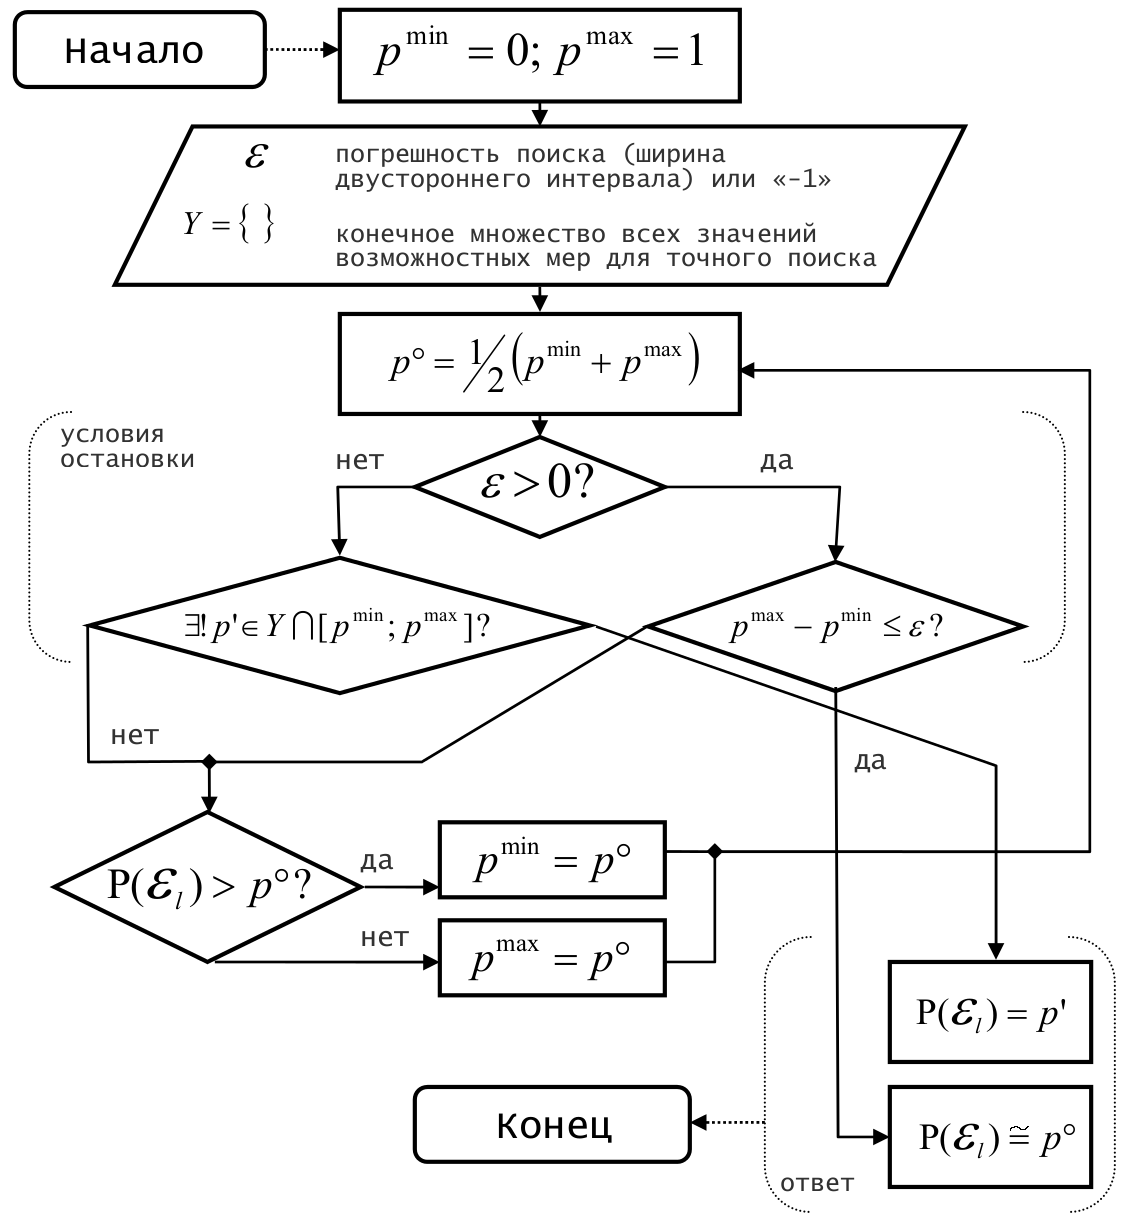
\includegraphics[width=0.75\linewidth]{./pic/block-scheme}}
\caption{\small Принципиальная блок-схема применяемого алгоритма дихотомии. Некоторые незначительне действия, например, расчёт максимального количество итераций и проверка на его достижение, здесь опущены. В зависимости от того, задано ли положительное значение $\varepsilon$ и множество всех значений возможностных мер $Y$, алгоритм может искать приближённое или точное значение $\P(\Eps_l)$. <<Сердцем>> алгоритма является проверка утверждения $\P(\Eps_l) > p$.}
\label{ris:algo_scheme}
\end{figure}

%Пусть на $N$-ой итерации дихотомии $p^{(N)} = p \in \zo$.
Пусть $p \in \zo$. <<Сердцем>> алгоритма является проверка утверждения $\P(\Eps_l) > p$. Чтобы узнать, верно ли это утверждение, выполним следующие действия: 
\begin{enumerate}
  \item 
  Для каждого $i \in \{1, ..., n\}$, $j \in \{1, ..., m\}$ найдём подмножество $X_{ij} \define= \{x \in X: p_{ij}(x) > p\} \subset X$. 
  \item 
  Определим $t^\text{edge} = (x_{11}^\text{edge}, \mydots, x_{nm}^\text{edge})$ следующим образом:
  \begin{equation*}
    x_{ij}^\text{edge} =
    \begin{cases}
      \min X_{ij}, &\text{если $i = l$.}\\
      \max X_{ij}, &\text{если $i \neq l$.} 
    \end{cases}
  \end{equation*}
  Элементарное событие, которому соотвествует вектор $t^\text{edge}$, заключается в том, что параметры $j$ объекта $l$ приняли минимальные значения среди $X_{lj}$, а каждый параметр $j$ всех остальных объектов $i \neq l$, наоборот, принял максимальное значение в <<своём>> множестве $X_{ij}$. 
  \item	%не совпадающих с $l$-м, %%ни фига, сверил с кодом
  Вычислим значение $\pi_l(t^\text{edge})$: 
 	\begin{itemize}
		\item если $\pi_l(t^\text{edge}) > k$, то $\P(\Eps_l) > p$.
		\item в противном случае, $\P(\Eps_l) \leq p$.
	\end{itemize} 
\end{enumerate}  

Проясним смысл этих действий. Поскольку в теории возможностей верно
\begin{equation*}
 % \label{e:transitive}
  \P(A) > a \Leftrightarrow \exists\, t \in A: \p(t) > a,
\end{equation*}
то в силу (\ref{e:pl_main}) утверждение $\P(\Eps_l) \leq p$ истинно, если и только если у всех векторов $t = \tvector \in \Eps_l$ хотя бы одна координата $x_{ij}$ такова, что $\p_{ij}(x_{ij}) \leq p$. Построим отрицание к сказанному: $\P(\Eps_l) > p$ истинно, если и только если найдётся хотя бы один вектор $t \in \Eps_l$, у которого все координаты $x_{ij} $ будут лежать в соответствующих подмножествах $X_{ij} = \{x \in X: p_{ij}(x) > p\}$, $i = \dotN$, $j = \dotM$.
%\begin{equation}
%  \label{e:P_greater_p}
%  \P(\Eps_l) > p \Leftrightarrow \exists\; t = (x_{11}, \mydots, x_{nm}) \in \Eps_l: \forall\; i = \dotN, j = \dotM  x_{ij} \in X_{ij} = \{x \in X: p_{ij}(x) > p\}.
%\end{equation}

Координаты $x_{ij}^\text{edge}$ вектора $t^\text{edge}$ по построению лежат в соответствующих подмножествах $X_{ij}$. Поэтому если $t^\text{edge} \in \Eps_l$, сразу делается вывод $\P(\Eps_l) > p$. Докажем, что если $t^\text{edge} \notin \Eps_l$, то и никакой другой вектор $t$ с координатами $x_{ij} \in X_{ij}$ не лежит в $\Eps_l$. 

Функция $\pi_l$ монотонно зависит от каждой координаты вектора $t \in T$ в силу монотонности $f$ по каждому аргументу: она невозрастает при возрастании той группы координат, которая обуславливает возрастание $x_l(t)$, и неубывает при возрастании всех остальных координат. По построению $t^\text{edge}$, изменение каких-либо из координат $x_{ij}^\text{edge}$ в пределах $X_{ij}$ не уменьшает $x_l(t^\text{edge})$ и не увеличивает $x_i(t^\text{edge}), i \neq l$. Поэтому вектору $t^\text{edge}$ соответствует максимально большое значение $\pi_l$ в пределах события $A = \{t = (x_{11}, ..., x_{nm}): x_{ij} \in X_{ij}\}$.

Событие $\Eps_l$ по определению состоит из $t: \pi_l(t) > k$, и либо пересекается, либо не пересекается с $A$, см.~рис.~\ref{ris:algo_sets}. Если $\Eps_l \cap A = \varnothing$, то их можно разделить прямой $\{\pi_l(t) = \pi_l(t^\text{edge})\}$, которая обозначена пунктиром на рисунке. Что и требовалось доказать.

\begin{figure}[h!]
\center{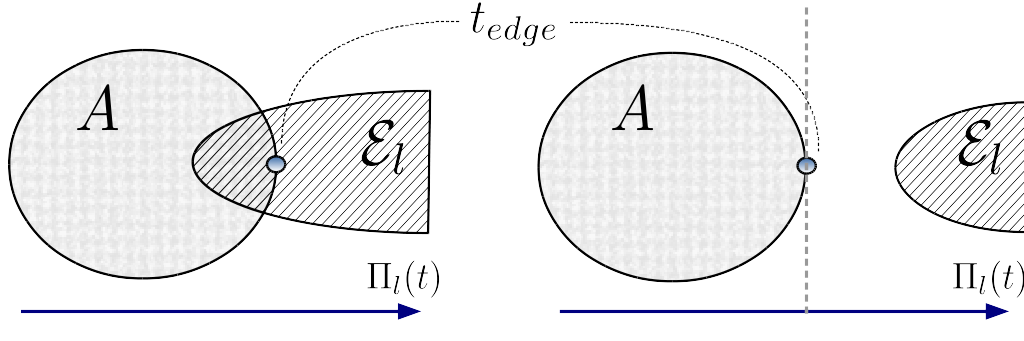
\includegraphics[width=0.85\linewidth]{./pic/algo_sets2}}
\caption{\small Иллюстрация взаимного расположения исследуемых событий и построенного вектора $t_{edge}$ в случае $\P(\Eps_l) > p$ (справа) и в случае $\P(\Eps_l) \leq p$ (слева) для заданного $p \in \zo$.}
\label{ris:algo_sets}
\end{figure}

%\subsection{Анализ корректности решения задачи выбора}
% ==moved up
\begin{comment}
\subsubsection*{Замечание 2}

Пусть $E_0 = \{t: \nexists \delta(t)\}$. Это событие возникает, когда найдётся хотя бы $n-k+1$ объектов, для каждого из которых найдётся $k$ объектов не меньшей <<значимости>>:
\begin{equation*}
 E_0 = (\Eps_1 \cap ... \cap \Eps_{n-k+1}) \bigcup (\Eps_2 \cap ... \cap \Eps_{n-k+2}) \bigcup ... \bigcup (\Eps_{k-1} \cap ... \cap \Eps_{n}).
 % надо было бы объедиение по всем возможным наборам, но всё гораздо проще!
\end{equation*}
Событие $E_0$ --- более узкое, чем $\Eps_l$, где требуется $k$ объектов не меньшей <<значимости>> только для объекта $l$:
\begin{equation*}
 E_0 \subset \Eps_l \Rightarrow \Eps_l = E_0 \cup E_l,\;l \in O,
\end{equation*}
где $E_0$ состоит из векторов $t: \nexists \delta(t)$, которые войдут во все $\Eps_l$, а 
$E_l$ --- оставшаяся часть $\Eps_l$. По правилу сложения возможностей:
\begin{equation*}
 \P(\Eps_l) = \sup\{\P(E_0), \P(E_l)\}.
\end{equation*}
%НЕ СОВСЕМ ВЕРНО: Постоянное первое слагаемое зависит, прежде всего, от выбора $f$ (\ref{e:function_f}). Если оно больше, чем минимум второго слагаемого, для некоторых $l$, возможности таких $\Eps_l$ будут равны, а это может быть плохо для однозначности решения задачи (\ref{e:zadacha}). Поэтому в спорной ситуации, когда в цепочке (\ref{e:left_order}) много равенств, имеет смысл посмотреть на возможность $\P(E_0)$. Если она окажется равна многим $\P(\Eps_l)$, требуется выбрать другую функцию $f$. Если же нет, то спорная ситуация возникла только из-за экспертных $\p_{ij}$.
\end{comment}
 
\clearpage
%\begin{comment}
\section{Задача нахождения оценки, выражающей коллективное мнение экспертов}
% Объединение возможностеи
\label{collective_global}

Если оценку параметров объектов $x_{ij}$ для задачи выбора объектов (см. раздел~\ref{selection_task}) совершают несколько экспертов, исходным материалом для программного комплекса служат оценки 
\begin{equation}
\label{Psetlargedef}
	\Pi_{ij} = \{\p^{(r)}\}_{ij}, i = \dotN, j = \dotM, r = \dotR, 
\end{equation}
где $r$ --- номер эксперта, $i$ --- номер объекта, $j$ --- номер параметра объекта. На вход алгоритма выбора объектов подаются только экспертное  мнение одного эксперта (см. рис.~\ref{ris:program_global}) $\p_{ij},  i = \dotN, j = \dotM$,  поэтому в настоящем разделе ставятся задачи сведения набора $\Pi_{ij}$ к $\p_{ij}$ для всех $i = \dotN, j= \dotM$ --- задачи нахождения  оценок, выражающих коллективное мнение экспертов, или, короче говоря, задачи <<коллективной экспертизы>>. 

\begin{figure}[h]
\center{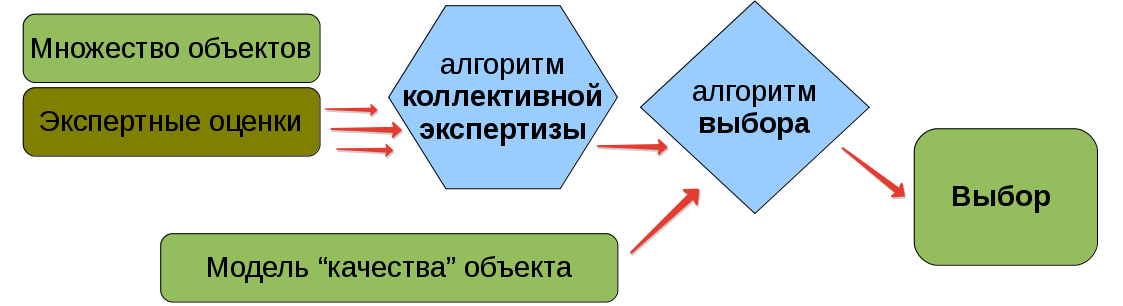
\includegraphics[width=0.85\linewidth]{./pic/globalscheme}}  
\caption{\small Схема, иллюстрирующая работу программного комплекса в режиме нахождения наиболее <<качественных>> объектов на выходе по мнениям нескольких экспертов и модели <<качества>> объектов (функции $f: x = f(x_1, x_2, ...)$) на входе. }
\label{ris:program_global}
\end{figure}

Задача коллективной экспертизы в рамках использования модели нечётких оценок в теории возможностей Пытьева может быть поставлена и решена различными методами:
	\begin{enumerate}
		\item Методы <<евклидовой близости к среднему>>~\cite{pytyev_experts}: метод матриц попарных сравнений, векторов перестановок, векторов предпочтений и др.;
		\item Новый метод -- введение отношения квазипорядка~\ref{preorder_pyt}  на множестве возможностных распределений нечётких  элементов $\tilde x_{ij}$ (см. раздел~\ref{selection_task}) и вычисление верхней (нижней) грани или точной верхней (нижней) грани каждого из множеств~\ref{Psetlargedef} экспертных оценок от разных экспертов, отдельно для каждого $i = \dotN, j= \dotM$.
	\end{enumerate} 
	
\subsection{Методы <<евклидовой близости к среднему>>}


	
\subsubsection{Метод матриц попарных сравнений}


\subsubsection{Метод векторов предпочтений}


\subsection{Метод вычисления верхних граней множеств экспертных оценок}

\subsubsection{Квазипорядок на множестве возможностных распределений}
\label{preorder_pyt}

Определение квазипорядка аналогично определению порядка \eqref{interv_order}, за исключением отсутствия требования равенства в качестве эквивалентности~\cite{Mirkin}: 
 \begin{equation}
\label{preoder_def}
\begin{split}
\forall A: & A \prec A; \\
\forall A, B, C: & A \prec B \text{ и } B \prec C \Rightarrow A \prec C.
\end{split}
\end{equation}

На множестве возможностных распределений, определённых на (одном и том же, фиксированном) множестве $X$, то есть на множестве функций $\p(\cdot):\ X\to[0,1]$, таких что $\sup_{x\in X} \p(x) = 1$, введём отношение~<<$\prec$>>: $\p_1\prec\p_2$, если:
\begin{enumerate}
    \item\label{order-D1}
        носитель $\p_1(\cdot)$ меньше (по включению), чем носитель $\p_2(\cdot)$: $\supp\p_1\subset\supp\p_2$;
    \item\label{order-D2}
        найдётся непрерывная строго монотонная функция ${\gamma(\cdot):\ [0,1]\to[0,1]}$, $\gamma(0) = 0$, $\gamma(1) = 1$, такая что $\p_2(x) = \gamma(\p_1(x))$ при $x\in\supp\p_1$;
    \item\label{order-D3}
        значения распределения $\p_2(\cdot)$ на носителе распределения $\p_1(\cdot)$ не меньше, чем значения $\p_2(\cdot)$ вне носителя $\p_1(\cdot)$:
        $$\inf\{\p_2(x) \mid x\in\supp\p_1\} \geqs \sup\{\p_2(x) \mid x\in X\setminus\supp\p_1\};$$
\end{enumerate}
где $\supp \p_i = \{x\in X:\ \p_i(x) > 0\}$~--- носитель распределения $\p_i(\cdot),\ i=1,\, 2$.

В ходе выполнения работы показано, что отношение <<$\prec$>> является отношением квазипорядка, то есть рефлексивно и транзитивно. При этом из $\p_1\prec\p_2$ и $\p_2\prec\p_1$ не следует тождественное равенство $\p_1(\cdot)$ и $\p_2(\cdot)$, однако из этого следует эквивалентность возможностных распределений $\p_1(\cdot)$ и $\p_2(\cdot)$, то есть существование непрерывной строго монотонной функции $\gamma(\cdot):\ [0,1]\to[0,1]$, $\gamma(0) = 0$, $\gamma(1) = 1$, такой что $\p_2(x) = \gamma(\p_1(x))$ при $x\in X$.

В случае, если распределения $\p_1(\cdot)$ и $\p_2(\cdot)$ сравнимы, то есть $\p_1\prec\p_2$ или $\p_2\prec\p_1$, будем говорить, что эти распределения не противоречат друг другу,
а запись $\p_1\prec\p_2$ будем читать как <<$\p_1$ уточняет $\p_2$>>.
Это связано с интерпретацией квазипорядка <<$\prec$>> как отношения, упорядочивающего возможностные распределения по степени их информативности. Такая интерпретация может быть проиллюстрирована тем, что всякое распределение, достигающее значения 1 в точке $x_0$, уточняет тривиальное распределение, тождественно равное единице, и одновременно с этим уточняется <<дельтобразным>> распределением, принимающим значение 1 в точке $x_0$ и значение 0 во всех остальных точках области определения.

\section{Содержательная интерпретация квазипорядка на множестве возможностных распределений}

Строгое обоснование содержательной интерпретации отношения <<$\prec$>> основано на его роли в следующей задаче принятия решений.

Пусть $\eta$ и $\zeta$~--- нечёткие элементы со значениями в $Y$ и $Z$ соответственно, совместное распределение возможностей которых есть $\p(\cdot):\ Y\times Z\to[0,1]$, и по реализации $y\in Y$ элемента $\eta$ требуется принять решение о реализации $z\in Z$ элемента $\zeta$. Множество чётких стратегий, минимизирующих возможность ошибки при $\p(\cdot) = \p_1(\cdot)$, обозначим $D_1$, при $\p(\cdot) = \p_2(\cdot)$~--- $D_2$.
В ходе выполнения работы доказана следующая теорема.

\begin{theorem}
\label{theorem_zubyuk}
    Пусть $\p_1\prec\p_2$, и множества $D_1$ и $D_2$ не пусты. Тогда при $\p(\cdot) = \p_1(\cdot)$ всем стратегиям из $D_1$ соответствует либо ненулевая возможность ошибки, при этом $D_1\subset D_2$, либо нулевая возможность ошибки, при этом для всякой $d_1\in D_1\setminus D_2$ найдётся такая стратегия $d_1'\in  D_1\cap D_2$, что возможность несовпадения решений, принятых с использованием $d_1$ и $d_1'$, равна нулю.
\end{theorem}

Рассмотрим подробно смысл данной теоремы. Итак, если всякой стратегии из множества $D_1$ соответствует ненулевая возможность ошибки, то $D_1\subset D_2$, то есть использование распределения $\p_1(\cdot)$ вместо $\p_2(\cdot)$ позволяет сузить множество оптимальных стратегий. Это в полной мере согласуется с трактовкой отношения $\p_1\prec\p_2$ как выражения того, что распределение $\p_1(\cdot)$ не менее информативно, чем $\p_2(\cdot)$: чем более информативно распределение, тем более конкретный ответ (более узкое множество оптимальных стратегий) оно позволяет получить в задаче принятия решений.

В случае, если всем стратегиям из множества $D_1$ соответствует нулевая возможность ошибки,
множество $D_1$, вообще говоря, не уже, чем множество $D_2$.
Однако для всякой стратегии $d_1\in D_1\setminus D_2$ в этом случае найдётся эквивалентная ей стратегия $d_1'\in D_1\cap D_2$; эквивалентность здесь понимается как равенство нулю возможности несовпадения принятых с использованием $d_1$ и $d_1'$ решений при $\p(\cdot) = \p_1(\cdot)$.
Таким образом, пополнение множества оптимальных стратегий при использовании распределения $\p_1(\cdot)$ вместо $\p_2(\cdot)$ может быть связано исключительно с тем, что некоторые элементарные исходы, имеющие ненулевую возможность при $\p(\cdot) = \p_2(\cdot)$, имеют нулевую возможность при $\p(\cdot) = \p_1(\cdot)$. Только при реализации таких исходов эквивалентные стратегии из множеств $D_1\setminus D_2$ и $D_1\cap D_2$ приводят к принятию разных решений.
Однако тот факт, что некоторые элементарные исходы, имеющие ненулевую возможность при $\p(\cdot) = \p_2(\cdot)$, имеют нулевую возможность при $\p(\cdot) = \p_1(\cdot)$ как раз и означает, что распределение $\p_1(\cdot)$ более информативно, чем $\p_2(\cdot)$: распределение $\p_1(\cdot)$ более конкретно, более чётко определяет исход эксперимента, так как множество возможных исходов при $\p(\cdot) = \p_1(\cdot)$ уже, чем при $\p(\cdot) = \p_2(\cdot)$.	
	
\subsubsection{Супремум и инфинум возможностных распределений. Алгоритм вычисления супремума}
\label{algo_sup_poss}

Для любой пары распределений $\p_1(\cdot)$ и $\p_2(\cdot)$ распределение $\p_1\vee\p_2(\cdot)$ определим как их супремум (если он существует), то есть как наиболее информативное среди всех распределений, уточняемых обоими распределениями $\p_1(\cdot)$ и $\p_2(\cdot)$. Распределение $\p_1\wedge\p_2(\cdot)$ определим как инфимум $\p_1(\cdot)$ и $\p_2(\cdot)$ (если он существует), то есть как наименее информативное среди всех распределений, уточняющих $\p_1(\cdot)$ и $\p_2(\cdot)$.

В ходе выполнения работы показано, что в случае, если область определения возможностных распределений конечна, супремум существует для любой пары распределений.  Тогда множество всех распределений образует полурешётку с идемпотентной, коммутативной, ассоциативной и дистрибутивной алгебраической операцией <<$\vee$>>, см. рис.~dummy. 
\begin{notive}
В случае, если область определения возможностных распределений конечна, инфимум тоже существует для любой пары распределений, если множество всех распределений пополнено функцией $0(\cdot)$, тождественно равной нулю на всей области определения (заметим, что с формальной точки зрения такая функция не является возможностным распределением, так как не найдётся точки, возможность которой равна 1). Более того, в ходе выполнения работы показано, что какой бы ни была область определения возможностных распределений, пополнение множества распределений функцией $0(\cdot)$ является необходимым условиям существования инфимума для любой пары распределений. Если для любой пары возможностных распределений существуют и супремум и инфимум, , множество всех распределений, пополненное $0(\cdot)$, образует решётку с алгебраическими операциями <<$\vee$>> и <<$\wedge$>>, являющимися идемпотентными, коммутативными, ассоциативными и дистрибутивными.
\end{notice}

Доказана система теорем, позволившая разработать численный метод построения супремума возможностных распределений и его компьютерную реализацию. А именно, алгоритм постоения супремума выглядит так.
dummy

\subsubsection{Супремум как коллективное мнение экспертов}

Теоретико-возможностная модель всех параметров всех объектов в задаче выбора определяется распределением $\p(\cdot):\ X\to[0,1]$ нечёткого вектора $\theta = \tetavector$, заданным формулой~\ref{p_theta_def}. Пусть из разных источников (от разных экспертов) получена информация, выраженная распределениями 
\begin{equation*}
	\p_r \big(\tvector\big) =  \inf_{i, j}\,\p^{(r)}_{ij}(x_{ij}), 
\end{equation*}
и на основе этой информации должно быть построено неизвестное распределение $\p$, являющееся по отношению к экспертным мнениям $\{\p_r\}$ коллективным мнением экспертов. 

Пусть множество всех распределений нечёткого элемента$\theta$, образует полурешётку с алгебраической операцией <<$\vee$>> (см. раздел~\ref{algo_sup_poss}). Поскольку операция <<$\vee$>> транзитивна и ассоциативна, можно, не ограничивая общности, положить $R = 2$, и тогда качестве коллективной экспертизы можно взять распределением $\p_1 \vee\p_2(\cdot)$, пользуясь алгоритмом из раздела~\ref{algo_sup_poss}. Рассмотрим содержательную сторону этого подхода.



Первый подход является математическим выражением принципа недоверия источникам информации. Он может быть применён в том случае, если хотя бы одно из распределений $\p_1(\cdot)$ и $\p_2(\cdot)$ уточняется распределением $\p(\cdot)$. То есть если информация, полученная из одного из источников, может противоречить истине, но при этом информация из другого источника истине не противоречит, но, вообще говоря, не полна. Покажем, что в этом случае означает использование распределения $\p_1\vee\p_2(\cdot)$ вместо $\p(\cdot)$ на примере задачи принятия решения о реализации $t$ нечёткого элемента $\theta$ по реализации $y$ нечёткого элемента $\eta$, рассмотренной выше. Обозначим $D$, $D_1$, $D_2$ и $D'$~--- множества стратегий, оптимальных в рамках моделей, определяемых распределениями $\p(\cdot)$, $\p_1(\cdot)$, $\p_2(\cdot)$ и $\p_1\vee\p_2(\cdot)$ соответственно. При выполнении указанных условий $\p\prec\p_1\vee\p_2$, $\p_1\prec\p_1\vee\p_2$ и $\p_2\prec\p_1\vee\p_2$. Пусть, для определённости, $D\subset D'$, $D_1\subset D'$ и $D_2\subset D'$, см. теорему~\ref{theorem_zubyuk}. Это означает, что множество $D'$ содержит все стратегии, оптимальные в рамках истинной модели. Однако кроме них она содержит также все стратегии, оптимальные в рамках моделей, соответствующих информации, полученной из обоих источников. То есть в множество $D'$ включаются все стратегии, оптимальные хотя бы для одного из $\p_i(\cdot),\ i=1,\, 2$, а те стратегии, которые нет оснований включить в множество $D'$ (с учётом информации, полученной из двух рассматриваемых источников), в него не включаются.

Второй подход является математическим выражением принципа доверия источникам информации. Он может быть применён в том случае, если оба распределения $\p_1(\cdot)$ и $\p_2(\cdot)$ уточняются распределением $\p(\cdot)$. То есть если информация из обоих источников не противоречит истине, но, вообще говоря, не полна. Как и выше, покажем, что в этом случае означает использование распределения $\p_1\wedge\p_2(\cdot)$ вместо $\p(\cdot)$ на примере задачи принятия решения о реализации $t$ нечёткого элемента $\theta$ по реализации $y$ нечёткого элемента $\eta$.
Обозначим $D$, $D_1$, $D_2$ и $D'$~--- множества стратегий, оптимальных в рамках моделей, определяемых распределениями $\p(\cdot)$, $\p_1(\cdot)$, $\p_2(\cdot)$ и $\p_1\wedge\p_2(\cdot)$ соответственно. При выполнении указанных условий $\p\prec\p_1\wedge\p_2$, $\p_1\wedge\p_2\prec\p_1$ и $\p_1\wedge\p_2\prec\p_2$. Пусть, для определённости, $D\subset D'$ и $D'\subset D_1\cap D_2$, см. теорему~\ref{theorem_zubyuk}.
Это означает, что множество $D'$ содержит все стратегии, оптимальные в рамках истинной модели. При этом в множество $D'$ включаются только те стратегии, которые оптимальны для обоих распределений $\p_1(\cdot)$ и $\p_2(\cdot)$, то есть все те стратегии, которые нет оснований не включить в $D'$ (с учётом информации, полученной из двух рассматриваемых источников).

%( два похода к объединению экспертных мнений -- вектор предпочтений и супремум. два применения всей этой техники -- коллективная экспертиза и диалог с экспертом)
\clearpage

\section{Комплекс программ для проведения экспертизы и пример его использования }

\label{sec:examples}

В ходе настоящей работы был создан комплекс программ для решения задачи выбора объектов, рассмотренной в разделе~\ref{selection_task}. Пользовательский интерфейс программного комплекса позволяет вводить экспертные оценки, задавать функцию <<качества>> объектов и т.\,д. Общая структура комплекса программ представлена на рис.~\ref{ris:program_global}, а скриншот пользовательского интерфейса представлен на рис.~\ref{ris:interface}.

Далее рассмотрим несколько модельных (искусственных) примеров использования описанных в настоящей работе методов, а затем --- пример реального проекта, где применялся комплекс программ и где предложенная методика проведения экспертного опроса использовалась крупным российским инвестором для оценки инвестиционной привлекательности технологий, разрабатываемых в МГУ.

\begin{figure}[h]
\center{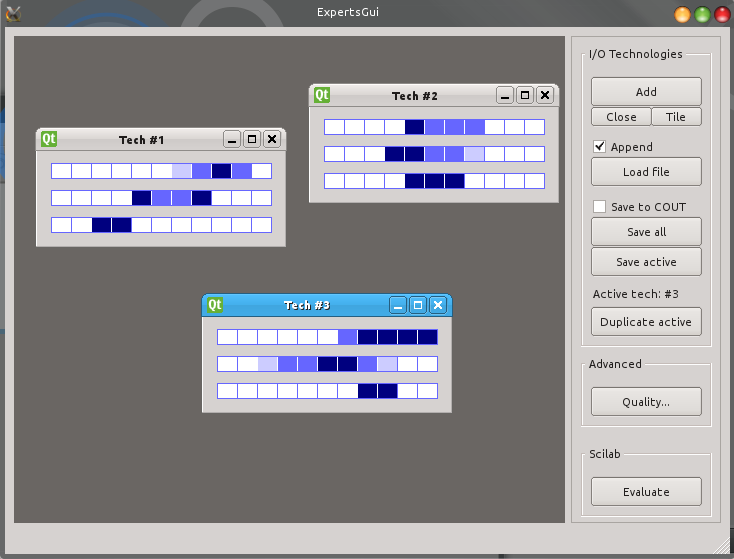
\includegraphics[width=0.85\linewidth]{./pic/combination6}}  
\caption{\small Скриншот пользовательсого интерфейса. Маленькие окошки соответствуют отдельным технологиям, а строчки квадратиков внутри них --- параметрам этих технологий. Сами квадратики символизируют баллы по шкале $X = \{0, 1, \ldots, 10\}$, а оттенок цвета конкретного квадратика --- возможность этого балла, по мнению эксперта (от белого, соответствующего возможности 0, до тёмно-синего, соответствующего возможности 1). }
\label{ris:interface}
\end{figure}

\subsection{Модельные примеры использования метдов, описанных в работе}

\subsection{Выбор наиболее привлекательных инновационных технологий}

%Этот пример построен вокруг реального проекта, где  %

Пусть имеется множество инновационных технологий $O$ размера $\abs{O} = N$.  Технология --- результат научно-технической деятельности, который включает в себя изобретения, промышленные образцы, компьютерные программы, технические данные или другие результаты интеллектуальной деятельности и может служить основой определённой практической, в том числе коммерческой деятельности. Каждая технология имеет одного или нескольких правообладателей, получающих выгоду от её применения в практической деятельности. Технологии являются инновационными в том смысле, что обладают значительной новизной и гипотетически имеют большой потенциал для развития, внедрения и получения прибыли, но всё это сопровождается значительным риском. 

%Если делать акцент не на самой технологии, а на команде людей, которые заняты разработкой и практическим применением технологии, то говорят об инновационном проекте или инновацонной компании. Всё, что ниже сказано про оценку технологий, остаётся верно и для оценки компаний с точностью до выбора критериев оценки.
%Есть крупный инвестор, у которого есть возможность стать совладельцем или полным владельцем технологии, если он вложит деньги и иные ресурсы в её развитие, вступив в сделку с текущими правообладателями. 
% (и так очевидно)

С точки зрения инвестора, технологии обладают разной инвестиционной привлекательностью, которая оценивается исходя из нескольких аспектов технологии, среди которых: доходность технологии через год после приобретения, её востребованность на рынке, конкурентоспособность, затраты на внедрение, потенциал интеллектуальной собственности, потенциал кадрового обеспечения, экологические риски, административные риски и т.\,д. 

Пусть привлекательность технологии по всем важным аспектам выражается числами $x_1 \in X_1, x_2 \in X_2, ...$, где мы для простоты положили $X_1 = X_2 = ... = \{0, ..., 10\}$. Инвестиционная привлекательность получается из этих чисел с помощью обычных операций сложения, перемножения и умножения на некоторые коэффициенты в соответствии со специально разработанной блок-схемой (рис.~\ref{ris:tech_scheme}), которая графически выражает функцию $f$, см. \eqref{e:function_f} на стр. \pageref{e:function_f}). 

\begin{figure}[h]
\center{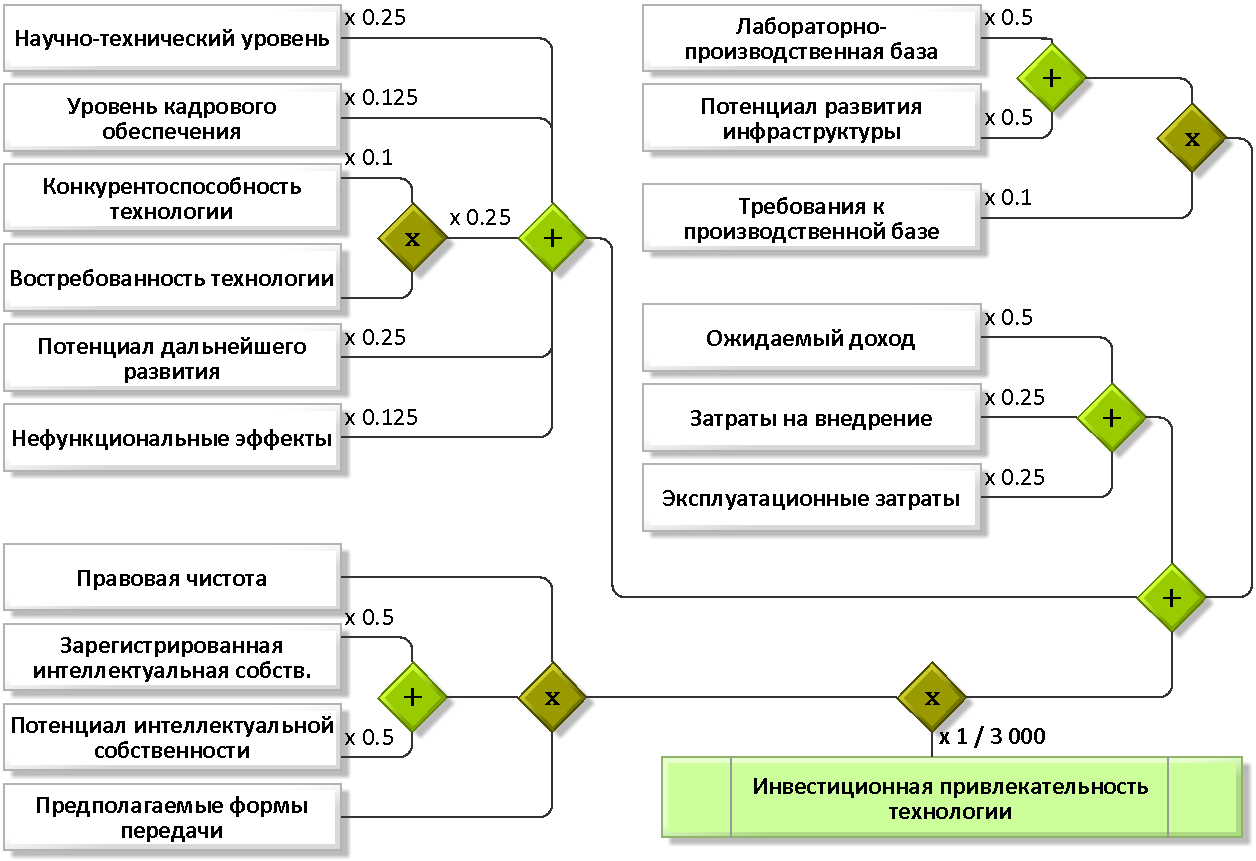
\includegraphics[width=0.85\linewidth]{./pic/schemeF2}}  
\caption{\small Блок-схема, иллюстрирующая конкретный вид функции $f$, объединяющей различные аспекты инновационной технологии, оцениваемые экспертом, в итоговую величину инвестиционной привлекательности технологии. }
\label{ris:tech_scheme}
\end{figure}

Были приглашены несколько экспертов. Каждого эксперта попросили оценить каждую технологию по каждому аспекту. Использовались нечёткие оценки, представленные в виде таблицы <<балл (значение $x \in \{0, ..., 10\}$) --- оценка (значение $p_{\tilde x}(x)$)>>, см.~рис.~\ref{ris:expert_sample}. В рассматриваемом случае выделялось $M = 16$ крупных аспектов с отдельными оценками. При этом с точки зрения методологии каждый из этих аспектов <<вобрал в себя>> ряд более мелких подпунктов примерно одинаковой важности, которые уже не требовали отдельных оценок во избежание чрезмерной нагрузки на эксперта. В документе-описании, который выдавался каждому эксперту, все аспекты расшифрованы: указано, какие подпункты мы рассматриваем и о чём следует  подумать перед выставлением оценки по каждому аспекту.
 
\begin{figure}[h]
\center{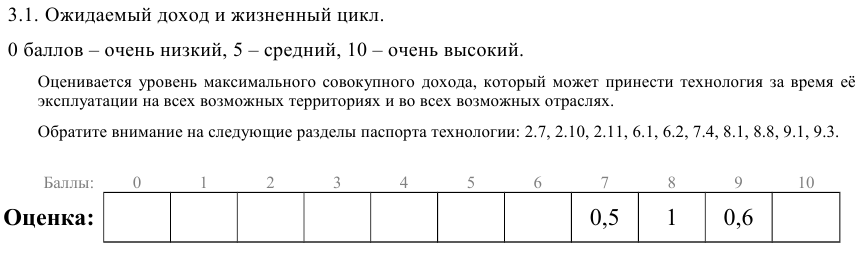
\includegraphics[width=0.85\linewidth]{./pic/expert_sample}}
\caption{\small Пример заполненного фрагмента листа экспертного опроса, проведённого по предложенной методике. Эксперт выставил нечёткую оценку в ячейках таблицы <<балл (значение $x$) --- оценка (значение $p(x)$)>>. Пустым клеткам таблицы соответствуют значения $p(x) = 0$. }
\label{ris:expert_sample}
\end{figure}

Интересно отметить, что для различных рисков и других негативных аспектов технологии большие числовые значения в таблице интуитивно соответствуют более плохой ситуации, более низкому <<качеству>> объекта. Но поскольку $f$ должна быть монотонна по всем аргументам, требуется единообразие, например, увеличение аргументов $f$  всегда приводит к более высокому значению $f$, т.\,е. более высокому <<качеству>>. Поэтому были сделалиы дополнительные указания для экспертов в тех местах, где большие числовые значения интерпретируются как более низкий риск. Этого можно избежать, если делать предварительную обработку оценок: автоматически отразить оценки, нарушающие монотонность, вдоль оси абсцисс (баллов) вокруг оси, проходящей через середину диапазона баллов.

Совокупность сырых экспертных оценок была загружена в программу расчёта коллективной оценки. Полученное коллективное мнение было загружено в программу, реализующую быстрый алгоритм нахождения возможности не попасть в $k$ лидеров для каждой из технологий, которых в рассматриваемом случае набралось $N = 15$ штук. Программа расчёта оптимального решения была запущена при разных значениях $k = 1, 2, \ldots, N$, в результате чего обнаружилось, что только при $k=2, 14$ можно сделать однозначный выбор технологий, опираясь на полученное оптимальное решение.  

Этот результат оправдал ожидания в следующем смысле. В рассмотриваемой ситуации выполнялся предварительных отбор <<плохох>> технологий, и на детальную экспертизу выносились технологии, приблизительно равные по ожидаемому экспертами <<качеству>>. Отсюда поятно, что большинство технологий-лидеров не разделяются по возможному <<качеству>> однозначно. В итоге получилось, что при желании выбрать небольшое число технологий-победителей для трансфера (покупки), разумно остановиться на $k=2$ технологиях. 


\begin{comment}
\subsection{Пример 2: Выбор оптимальных реактивов для маркировки белков в цикле ***}

Этот пример посвящён важной области применения экспертных опросов на стыке естественных наук и экономики --- области планирования эксперимента. 

Одним из центральных вопросов для науки биохимии является вопрос о том, какие химические реакции протекают в живом организме, и какие вещества участвуют в этих реакциях. Как правило, исследуют т.\,н. циклы реакций с участием белков. В живом организме встречается много тысяч различных белков и добрая сотня из них участвует в исследуемом цикле реакций. Концентрация веществ, участвующих в реакциях, в частности -- белков, как правило, изменяется на отдельных стадиях цикла реакций, и может изменяться в результате полного цикла.

Для идентификации конкретного белка и определения его концентрации служат специальные реактивы, причём один реактив может обладать активностью сразу к нескольким белкам (и заранее неизвестно, к каким?). Биологи контролируют изменение концентрации выбранных белков в некоторой точке организма таким образом, что организм не погибает (и вмешательство в его работу минимально?) По каждому белку есть предположения относительно того, насколько возможно, что: (1) его количество уменьшится, (2) не изменится, (3) увеличится. В силу некоторых причин, в том числе, но не ограничиваясь дороговизной реактивов, мы можем контролировать только небольшое количество белков, как правило, в пределах $10$.

Объекты -- белки. <<Качество>> белка складывается из того, какие белки, по мнению эксперта, участвуют в цикле (и их имеет смысл контролировать), и насколько дорогой реактив требуется для контроля. Эксперт оценивает для каждого белка $i \in \setN$ возможность $\p_{ij}(x)$ обнаружения изменения его концентрации на $x$ процентов (или чего там, логарифма какого-нибудь) с помощью реактива $j \in \setM$. Цены различных реактивов учтены в $f(\cdot)$ как коэффициенты перед $x_{ij}$ для разных $j$.

%Объекты -- реактивы. <<Качество>> реактивов складывается из того, какие белки, по мнению эксперта, участвуют в цикле. Эксперт оценивает для каждого реактива $i \in \setN$ возможность $\p_{ij} обнаружения каждого белка $j \in \setM$ (довольно много оценок, трудно для эксперта?). Нечёткий вектор $\theta: \p_{\theta} = \inf \p_{ij}$ не имеет смысла, т.\,к. (а) я забыл про баллы, ещё одно измерение и (б) при таком выборе нет независимости компонент, потому что есть априорные возможности обнаружить белок в реакции идеальным реактивом.    

%Выбор измерительного прибора мы будем рассматривать в контексте теории измерительно-вычислительнх преобразователей как средств измерений (ИВП) Ю.~П.~Пытьева \cite{4}. 
\end{comment}



\clearpage

\section{Заключение}
 
В настоящей работе рассмотрены задачи, связанные с  использованием экспертных оценок в форме распределений возможности в рамках теории возможностей Ю.~П.~Пытьева (такие оценки были названы нечёткими). В рамках упомянутой теории были впервые получены следующие результаты:
\begin{enumerate}
\item
Поставлена и решена задача принятия решения о выборе наиболее качественных объектов на основе нечётких экспертных данных об их характеристиках, сформулированная как задача на минимум возможности принять неверное решение (ошибиться);
\item
Поставлена и решена задача нахождения коллективного мнения экспертов, не противоречащего мнениям отдельных экспертов, сформулированная как задача нахождения верхней грани на множестве возможностных распределений (экспертных оценок), заданных экспертами, используя введённое на множестве распределений отношение квазипорядка.
\item 
\todo[inline]{Сократи этот пункт, не надо ничего лишнего. Например: разработан численный метод ..., позволивший решать данную задачу за время порядка O(...) вместо O(...) при использовании метода полного перебора, где $n$~--- ..., $m$~--- ...}
 \todo{Разработан}Привёден численный метод решения \todo{Напиши полностью --- задачи о выборе наиболее кач. об.}задачи пункта~(1), который оказывается вычислительно эффективным благодаря эффективности операций <<$\sup$>> и <<$\inf$>> в качестве сложения и умножения значений возможности соответственно. В задаче имеется, возможно, большое число  $n$ оцениваемых объектов, каждый из которых имеет $m$ параметров, из которых складывается качество $x \in X$ того или иного объекта. Предложенный алгоритм позволяет в случае конечного $X$ вычислить значение возможности ошибки за $O(nm)$ итераций вместо $O(\abs{X}^{nm})$ в случае полного перебора всех элементраных событий (тут $\abs{X}$ есть размер множества $X$).
 \item
 \todo{Здесь тоже кратче и чётче.}Предложен эвристический численный метод решения задачи \todo{нахождения коллективного мнения экспертов}пункта~(2), оказывающийся вычислительно эффективным за счёт отказа от вычисления точной верхней грани в пользу <<не слишком сильно>> отличающейся от неё верхней грани. Для тех же, возможно, больших чисел $n$, $m$ вычисления проводятся не с совместнымым распределениями возможности всех параметров всех объектов, что имело бы сложность $O(\abs{X}^{2nm})$, а с некоторыми искусственно полученными распределениями --- <<комбинациями>> маргинальных распределений, что позволяет снизить сложность алгоритма до $O((nm)^2)$.   
\end{enumerate}

\clearpage
%\end{comment}
% Список литературы
\printbibliography[heading=bibintoc]

\end{document}
